\chapter{More on Coordinate Bases, Linear Transformations}

In this chapter we will go deeper about what actually a matrix represents in the big picture. Matrices by nature is a rule of \textit{linear transformation} (or \textit{linear mapping}) between two vector spaces. We are going to study several special types of linear transformations, which ultimately reveals the relationship between any $n$-dimensional real vector space and the real $n$-space $\mathbb{R}^n$, as an \textit{isomorphism}. We then move to discuss how a change of coordinates works for vectors and matrices, as well as the \textit{Gram-Schmidt} process to make an \textit{orthonormal} basis.

\section{About Linear Transformations}

\subsection{Linear Maps between Vector Spaces}

Consider two vector spaces, we may want to know if vectors in one of the spaces, let's say $\mathcal{U}$, can be associated to or transformed into those in another vector space, $\mathcal{V}$, according to some rules. This is known as a \index{Transformation}\index{Transformation!Mapping}\keywordhl{transformation/mapping} from the vector space $\mathcal{U}$ to $\mathcal{V}$. Of the most concern is the class of \index{Linear Transformation}\index{Linear Transformation!Linear Mapping}\keywordhl{linear transformations/mappings} which obeys the two properties listed below.
\begin{defn}[Linear Transformation/Map]
\label{defn:lintrans}
A linear transformation (or linear map) from a vector space $\mathcal{U}$ to another vector space $\mathcal{V}$ is a mapping: $T: \mathcal{U} \to \mathcal{V}$, such that for all vectors $\vec{u}_1, \vec{u}_2 \in \mathcal{U}$, and any scalar $a$, it satisfies:
\begin{enumerate}
    \item $T(\vec{u}_1 + \vec{u}_2) = T(\vec{u}_1) + T(\vec{u}_2)$ (Additivity), and
    \item $T(a\vec{u}_j) = aT(\vec{u}_j)$ (Homogeneity).
\end{enumerate}
These two properties combined are known as \textit{linearity}. An equivalent condition is $T(a\vec{u}_1 + b\vec{u}_2) = aT(\vec{u}_1) + bT(\vec{u}_2)$, where $b$ is any scalar as well.
\end{defn}
Notice that if $\mathcal{U}$/$\mathcal{V}$ coincides with the real $n$/$m$-space $\mathbb{R}^n$/$\mathbb{R}^m$, and we express any vector $\vec{u}$: $[\vec{u}]_B$ in $\mathcal{U}$ with $n$ coordinates using some basis $\mathcal{B}$ of its (similarly for $\vec{v}$: $ [\vec{v}]_{H}$ in $\mathcal{V}$ having $m$ coordinates from some basis $\mathcal{H}$). Then $T$: $[T]_B^{H} = A$ where $A$ is any $m \times n$ matrix satisfies the requirements of and is a linear transformation from $\mathcal{U}$ to $\mathcal{V}$ according to the rule $T(\vec{u})$: $A[\vec{u}]_B$. (Short Exercise: show this satisfies the conditions outlined in Definition \ref{defn:lintrans}!\footnote{$T(\vec{u}_1+\vec{u}_2)$: $A([\vec{u}_1]_B + [\vec{u}_2]_B) = A[\vec{u}_1]_B + A[\vec{u}_2]_B$: $T(\vec{u}_1)+T(\vec{u}_2)$ and $T(a\vec{u}_1)$: $A(a[\vec{u}_1]_B) = a(A[\vec{u}_1]_B)$: $aT(\vec{u}_1)$}) This implies that all matrices can be considered as some sort of linear mappings (for now, between $\mathbb{R}^n$ and $\mathbb{R}^m$). In fact, the converse, which states that any linear transformation (between finite-dimensional vector spaces) can be represented by a matrix, is also true as well, and will be discussed in the remaining parts of this section.\\
\\
Let's now explicitly fix a basis $\mathcal{B} = \{\vec{u}_1, \vec{u}_2, \ldots, \vec{u}_n\}$ for $\mathcal{U}$ (again, similarly we have $\mathcal{H} = \{\vec{v}_1, \vec{v}_2, \ldots, \vec{v}_m\}$ for $\mathcal{V}$). For each $\vec{u}_j$, denote $\vec{v}^{(j)} = T(\vec{u}_j)$ as the resulting vectors in $\mathcal{V}$ after applying the transformation $T$ over the basis vectors for $\mathcal{U}$. Notice that $[\vec{u}_j]_B = (e_j)_B$ where the $j$-th basis vector of $\mathcal{B}$ is explicitly represented in a numeric tuple form with the $j$-th entry being $1$ and others being $0$ (where the usual hat symbol on $e$ is not present) in the $\mathcal{B}$ system. Due to Definition \ref{defn:coordRn} and Properties \ref{proper:lincombofspan}, $T(\vec{u}_j) = \vec{v}^{(j)}$ can be expressed as a unique linear combination as $\vec{v}^{(j)} = a_1^{(j)}\vec{u}_1 + a_2^{(j)}\vec{u}_2 + \cdots a_m^{(j)}\vec{u}_m = \sum_{i=1}^{m} a_i^{(j)}\vec{u}_i$ of the basis vectors $\vec{v}_i$ from $\mathcal{H}$, i.e.
\begin{align*}
T(\vec{u}_j) = \sum_{i=1}^{m} a_i^{(j)}\vec{v}_i
\end{align*}
The matrix formed by the above coefficients $A = a_i^{(j)}$ is then the desired \index{Linear Transformation!Matrix Representation of Linear Transformation}\keywordhl{matrix representation} of our linear transformation $T$. To see this, compare with what we have taken in the last paragraph, $T(\vec{u})$: $[\vec{u}]_B$. Subsequently,
\begin{align*}
T(\vec{u_j})\text{: } A[\vec{u}_j]_B &= a_i^{(j)}(e_j)_B \\
&=
\begin{bmatrix}
a_1^{(1)} & a_1^{(2)} & \cdots & a_1^{(j)} & \cdots & a_1^{(n)} \\
a_2^{(1)} & a_2^{(2)} & & a_2^{(j)} & & a_2^{(n)} \\
\vdots & & & \vdots & & \vdots \\
a_m^{(1)} & a_m^{(2)} & \cdots & a_m^{(j)} & \cdots & a_m^{(n)}
\end{bmatrix}
\begin{bmatrix}
0 \\
0 \\
\vdots \\
1 {\scriptsize \text{ (the $j$-th entry)}} \\
\vdots \\
0 {\scriptsize \text{ (the last index is $n$)}}
\end{bmatrix} \\
&=
\begin{bmatrix}
a_1^{(j)} \\
a_2^{(j)} \\
\vdots \\
a_m^{(j)}
\end{bmatrix}
\end{align*}
Due to the structure of $(e_j)_B$, this matrix product yields exactly the $j$-th column of $A = a_i^{(j)}$ as shown above (see Properties \ref{proper:linearcombmatrix}). Moreover, the coordinates of $\vec{v}^{(j)}$ in the $\mathcal{H}$ system
\begin{align*}
[\vec{v}^{(j)}]_H = [\sum_{i=1}^{m} a_i^{(j)}\vec{v}_i]_H &= \sum_{i=1}^{m} a_i^{(j)}[\vec{v}_i]_H \\
&= \sum_{i=1}^{m} a_i^{(j)}(e_i)_H \\
&=  a_1^{(j)} \begin{bmatrix}
1 \\
0 \\
\vdots \\
0
\end{bmatrix}
+
a_2^{(j)} \begin{bmatrix}
0 \\
1 \\
\vdots \\
0
\end{bmatrix}
+ \cdots
+
a_m^{(j)} \begin{bmatrix}
0 \\
0 \\
\vdots \\
1 {\scriptsize \text{ (the last index is $m$)}}
\end{bmatrix}
\\
&= \begin{bmatrix}
a_1^{(j)} \\
0 \\
\vdots \\
0
\end{bmatrix}
+
\begin{bmatrix}
0 \\
a_2^{(j)} \\
\vdots \\
0
\end{bmatrix}
+ \cdots
+
\begin{bmatrix}
0 \\
0 \\
\vdots \\
a_m^{(j)}
\end{bmatrix}
=
\begin{bmatrix}
a_1^{(j)} \\
a_2^{(j)} \\
\vdots \\
a_m^{(j)}
\end{bmatrix}
\end{align*}
also gives the same $j$-th column of $A = a_i^{(j)}$. This holds for any $j$. Hence, the association of the matrix $[A]_B^H = a_i^{(j)}$ to the linear transformation $T$ is consistent, where we have now added the subscript $B$ and superscript $H$ to emphasize the transformation are carried out in reference to the two specific coordinate bases. This reasoning also shows that, to construct the matrix representation of a linear transformation, we compute each of the $T(\vec{u}_j) = \vec{v}^{(j)}$ and find its coordinates in the $\mathcal{H}$ frame, namely $[\vec{v}^{(j)}]_H$, which readily become the $j$-th column of the matrix to be found. To be more clear, we have
\begin{align*}
[T]_B^H &= 
\begin{bmatrix}
[T(\vec{u}_1)]_H | [T(\vec{u}_2)]_H | \cdots | [T(\vec{u}_n)]_H
\end{bmatrix} \\
&=
\begin{bmatrix}
[\vec{v}^{(1)}]_H | [\vec{v}^{(2)}]_H | \cdots | [\vec{v}^{(n)}]_H
\end{bmatrix} \\
&= 
\begin{bmatrix}
a_1^{(1)} & a_1^{(2)} & \cdots & a_1^{(n)} \\
a_2^{(1)} & a_2^{(2)} &  & a_2^{(n)} \\
\vdots & & \ddots & \vdots \\
a_m^{(1)} & a_m^{(2)} & \cdots & a_m^{(n)}
\end{bmatrix}
= a_i^{(j)} = [A]_B^H
\end{align*}
Notice that here the $i$/$j$ subscript/superscript has been exchanged when compared to like Properties \ref{proper:linsysmat}.
\begin{defn}[Matrix Representation of a Linear Transformation]
\label{defn:matrixrepoflintrans}
A linear transformation $T: \mathcal{U} \to \mathcal{V}$ as defined in Definition \ref{defn:lintrans}, with respect to the bases $\mathcal{B} = \{\vec{u}_1, \vec{u}_2, \ldots, \vec{u}_n\}$ for $\mathcal{U}$ and $\mathcal{H} = \{\vec{v}_1, \vec{v}_2, \ldots, \vec{v}_m\}$ for $\mathcal{V}$, has a matrix representation of
\begin{align*}
[T]_B^H = 
\begin{bmatrix}
a_1^{(1)} & a_1^{(2)} & \cdots & a_1^{(n)} \\
a_2^{(1)} & a_2^{(2)} &  & a_2^{(n)} \\
\vdots & & \ddots & \vdots \\
a_m^{(1)} & a_m^{(2)} & \cdots & a_m^{(n)}
\end{bmatrix}
\end{align*}
where the entries $a_i^{(j)}$ are those according to the relations $T(\vec{u}_j) = \sum_{i=1}^{m} a_i^{(j)}\vec{v}_i$, or in matrix notation, $[T]_B^H [\vec{u}]_B = [\vec{v}]_H$.
\end{defn}

Let's illustrate how it works out using an easy example using the familiar $\mathbb{R}^n$ and $\mathbb{R}^m$. 
\begin{exmp}
\label{exmp:lineartransmatrixrep}
Let $\mathcal{U} = \mathbb{R}^3$ and $\mathcal{V} = \mathbb{R}^2$, it can be easily verified that $\mathcal{B} = \{(1,2,1)^T, (0,1,-1)^T, (2,-1,1)^T\}$ is a basis for $\mathcal{U}$, and the same goes for $\mathcal{V}$ with a basis $\mathcal{H} = \{(1,2)^T, (2,-1)^T\}$. If a linear transformation $T: \mathbb{R}^3 \to \mathbb{R}^2$ obeys the rule $T((x,y,z)^T) = (x+2y, x-y+z)^T$, (By the way, you should verify if this is really a linear transformation.) find its matrix representation $[T]_B^H$ with respect to $\mathcal{B}$ and $\mathcal{H}$. Then, use the results to compute $T((-1,4,-1)^T)$.
\end{exmp}
\begin{solution}
Following Definition \ref{defn:matrixrepoflintrans}, we set out to find how the linear transformation will apply on the basis vectors in $\mathcal{B}$. For the first one, we have
\begin{align*}
T((1,2,1)^T) = ((1)+2(2), (1)-(2)+(1))^T = (5,0)^T
\end{align*}
which can be subsequently written as a linear combination of the two basis vectors in $\mathcal{H}$:
\begin{align*}
(5,0)^T = 1(1,2)^T + 2(2,-1)^T
\end{align*}
Hence $a_1^{(1)} = 1$, $a_2^{(1)} = 2$, and this gives us the first column of $[T]_B^H$ as
\begin{align*}
\begin{bmatrix}
1 & * & * \\
2 & * & * 
\end{bmatrix}
\end{align*}
We repeat the same procedure on the other two basis vectors $(0,1,-1)^T$ and $(2,-1,0)^T$ of $\mathcal{B}$, where it can be shown that
\begin{align*}
T((0,1,-1)^T) &= ((0)+2(1), (0)-(1)+(-1))^T = (2,-2)^T \\
&= -\frac{2}{5}(1,2)^T + \frac{6}{5}(2,-1)^T \\
T((2,-1,1)^T) &= ((2)+2(-1), (2)-(-1)+(1))^T = (0,4)^T \\
&= \frac{8}{5}(1,2)^T - \frac{4}{5}(2,-1)^T
\end{align*}
Therefore, the required matrix representation is
\begin{align*}
[T]_B^H = 
\begin{bmatrix}
1 & -\frac{2}{5} & \frac{8}{5} \\
2 & \frac{6}{5} & -\frac{4}{5}
\end{bmatrix}
\end{align*}
For the second part, we start by expressing $(-1,4,1)^T$ in the basis $\mathcal{B}$. As $(-1,4,-1)^T = 1(1,2,1)^T + 1(0,1,-1)^T - 1(2,-1,1)^T$, we have $(-1,4,1)^T$: $(1,1,-1)_B^T$, and then
\begin{align*}
[T((1,1,-1)_B^T)]_H &= [T]_B^H (1,1,-1)_B^T \\
&=
\left(\begin{bmatrix}
1 & -\frac{2}{5} & \frac{8}{5} \\
2 & \frac{6}{5} & -\frac{4}{5}
\end{bmatrix}
\begin{bmatrix}
1 \\
1 \\
-1
\end{bmatrix}\right)_H \\
&=
\begin{bmatrix}
-1 \\
4
\end{bmatrix}_H = (-1,4)^T_H
\end{align*}
implying that $T((-1,4,-1)^T) = -1(1,2)^T + 4(2,-1)^T = (7,-6)^T$ in the usual standard basis. This can be cross-checked by directly invoking the given definition of $T$, where $T((-1,4,-1)^T) = ((-1)+2(4), (-1)-(4)+(-1))^T = (7,-6)^T$ as well.
\end{solution}

Up until now, we have been playing around with the simple real $n$-space only, but the real (no pun intended) power of the notion of a general vector space lies in its abstraction: Any mathematical object that satisfies the criteria in Definition \ref{defn:realvecspaceaxiom} is a (real) vector space, and the results that we have already established in the previous parts for the real $n$-space are readily transferable to them. Two prime examples of abstract vector spaces are the set of (real) polynomials $\mathcal{P}^n$ with a degree up to $n$ and\footnote{We shall argue for some criteria in Definition \ref{defn:realvecspaceaxiom} for $\mathcal{P}^n$ here. For instances, condition (1) is obvious as adding up two polynomials with a degree up to $n$ can only result in another polynomial with a maximum degree of $n$. In condition (4), the zero vector for $\mathcal{P}^n$ is simply the constant zero function $0$, which is considered to have a degree of $-1$ by convention.} the family of continuous ($k$-times continuously differentiable) functions $\mathcal{C}^0$ ($\mathcal{C}^k$) over a fixed interval. Now we will see how the concept of linear transformation is laid out when these abstract vector spaces are involved, preparing us for the key insight in the next subsection.

\begin{exmp}
\label{exmp:lineartransderivative}
Consider $\mathcal{U} = \mathcal{P}^2$, and $\mathcal{V} = \mathcal{P}^1$, and let the bases for $\mathcal{U}$ and $\mathcal{V}$ be $\mathcal{B} = \{1, x, x^2\}$ and $\mathcal{H} = \{1, x\}$. (They are known as the standard bases for $\mathcal{P}^2$ and $\mathcal{P}^1$ respectively. In general the standard basis for $\mathcal{P}^n$ is $\{1, x, x^2, \cdots, x^{n-1}, x^n\}$ and thus $n+1$-dimensional. Readers are advised to justify why they constitute a basis for the polynomial spaces.) Let $T: \mathcal{U} \to \mathcal{V}$ be $T[p(x)] = p'(x)$ the differentiation operator and find its matrix representation with respect to $\mathcal{B}$ and $\mathcal{H}$.
\end{exmp}
\begin{solution}
We essentially do the same thing as in Example \ref{exmp:lineartransmatrixrep} but applied over polynomials now. From elementary calculus, we have
\begin{align*}
T(1) &= \frac{d}{dx}(1) = 0 \\
T(x) &= \frac{d}{dx}(x) = 1 \\
T(x^2) &= \frac{d}{dx}(x^2) = 2x
\end{align*}
and by Definition \ref{defn:matrixrepoflintrans}, the desired matrix representation is
\begin{align*}
[T]_B^H = 
\begin{bmatrix}
0 & 1 & 0 \\
0 & 0 & 2
\end{bmatrix}
\end{align*}
Notice that we can express, quite trivially
\begin{align*}
1 &= \begin{bmatrix}
1 \\
0 \\
0
\end{bmatrix}_B
=
\begin{bmatrix}
1 \\
0
\end{bmatrix}_H \\
x &= \begin{bmatrix}
0 \\
1 \\
0
\end{bmatrix}_B
=
\begin{bmatrix}
0 \\
1
\end{bmatrix}_H \\
x^2 &= \begin{bmatrix}
0 \\
0 \\
1
\end{bmatrix}_B
\end{align*}
using vector notation in the given two standard bases. We can verify the form of $[T]_B^H$ by a test polynomial $c_0 + c_1x + c_2x^2$, whose vector representation in $\mathcal{B}$ is clearly $(c_0, c_1, c_2)^T_B$. Then, multiplying $[T]_B^H$ to its left gives
\begin{align*}
[T((c_0, c_1, c_2)^T_B)]_H = 
\begin{bmatrix}
0 & 1 & 0 \\
0 & 0 & 2
\end{bmatrix}_B^H 
\begin{bmatrix}
c_0 \\
c_1 \\
c_2
\end{bmatrix}_B
=
\begin{bmatrix}
c_1 \\
2c_2
\end{bmatrix}_H
\end{align*}
which corresponds to the polynomial $c_1 + 2c_2x$. This coincides with the usual result of differentiation, that is, $\frac{d}{dx}(c_0 + c_1x + c_2x^2) = c_1 + 2c_2x$.
\end{solution}

In each of the previous examples, we consider a linear transformation between two vector spaces that are of the same type (the usual real vectors/polynomials). Below shows what happen when they are mixed together. Actually, due to the abstraction provided by the nature of vector space, the outcome follows easily.
\begin{exmp}
Let $\mathcal{U} = \mathbb{R}^3$ and $\mathcal{V} = \mathcal{P}^2$, while $\mathcal{B} = \{(1,0,0)^T, (0,1,0)^T, (0,0,1)^T\}$ and $\mathcal{H} = \{1, x, x^2\}$ be the standard bases for $\mathcal{U}$ and $\mathcal{V}$ respectively. Show that, the rather trivial linear transformation $T((c_0, c_1, c_2)^T) = c_0 + c_1x + c_2x^2$ has a matrix representation of an identity with respect to $\mathcal{B}$ and $\mathcal{H}$.
\end{exmp}
\begin{solution}
Again, we repeat what we have done in the previous two examples. It is apparent that
\begin{align*}
T((1,0,0)^T_B) &= (1) + (0)x + (0)x^2 = 1 = (1,0,0)^T_H\\
T((0,1,0)^T_B) &= (0) + (1)x + (0)x^2 = x = (0,1,0)^T_H\\
T((0,0,1)^T_B) &= (0) + (0)x + (1)x^2 = x^2 = (0,0,1)^T_H
\end{align*}
So by Definition \ref{defn:matrixrepoflintrans}, the desired matrix representation is simply
\begin{align*}
[T]_B^H = 
\begin{bmatrix}
1 & 0 & 0 \\
0 & 1 & 0 \\
0 & 0 & 1
\end{bmatrix}
\end{align*}
which is the $3 \times 3$ identity matrix. This is expected as the linear transformation is essentially $T[(c_0, c_1, c_2)_B^T] = (c_0, c_1, c_2)_H^T$ where $(c_0, c_1, c_2)_H^T = c_0 + c_1x + c_2x^2$, which means that the numeric representation of vectors in the two spaces is preserved under such a linear transformation between them and the only visible change is the subscript.
\end{solution}
Most of the readers should find it boring in the above example as we are just stating the obvious. It is a straight-forward, "one-to-one" association between the standard bases of the real $n$-space and space of polynomials with degree $n-1$. However, the important message is that given such an association we can always identify any vector of some space as a vector in another space of a completely different class, which is very powerful as many operations become transferable between these two spaces. In this sense, this kind of "one-to-one" mapping is not limited to the identity mapping, or by the bases used for the two vector spaces as we will see in the following subsection.

\subsection{One-to-one and Onto, Kernel and Range}

Continuing our discussion above, to identify a vector (one and only one) from one vector space as another vector in another vector space through a linear mapping, we require it to be \index{One-to-one}\index{Injective}\keywordhl{one-to-one (injective)}. On the other hand, another important property of a linear transformation is that whether it is \index{Onto}\index{Surjective}\keywordhl{onto (surjective)}, which means that every vector in the latter vector space (\textit{image}) is being mapped onto by some vector(s) in the former vector space (\textit{preimage}). The formal definitions of these two properties are given as below.

\begin{proper}[Injective Transformation]
\label{proper:injective}
A transformation $T: \mathcal{U} \to \mathcal{V}$ is called one-to-one if for two vectors $\vec{u}_1, \vec{u}_2 \in \mathcal{U}$, $T(\vec{u}_1) = T(\vec{vu}_2)$ implies $\vec{u}_1 = \vec{u}_2$, i.e. an image has one and only one corresponding preimage. Furthermore, if $T$ is linear, then equivalently $T(\vec{u}) = \textbf{0}$ implies $\vec{u} = \textbf{0}$ only.
\end{proper}
To show the equivalence of the two conditions above, notice that $T(\textbf{0}) = \textbf{0}$ if $T$ is linear. (why?)\footnote{$T(\textbf{0})=T(0\vec{u})=0T(\vec{u})=\textbf{0}$ for arbitrary $\vec{v}$ due to the homogeneity property as required in Definition \ref{defn:lintrans}.} For any $\vec{v}$ such that $T(\vec{v}) = 0$, we have
\begin{align*}
T(\vec{v}) = \textbf{0} = T(\textbf{0})
\end{align*}
and hence $\vec{v}$ must be $\textbf{0}$ if $T(\vec{v}_1) = T(\vec{v_2})$ implies $\vec{v}_1 = \vec{v}_2$. The proof of the converse is left as an exercise.
\begin{proper}[Surjective Transformation]
\label{proper:surjective}
A transformation $T: \mathcal{U} \to \mathcal{V}$ is called onto if for any vector $\vec{v} \in \mathcal{V}$ (image), there exists at least one vector(s) $\vec{u} \in \mathcal{U}$ (preimage) such that $T(\vec{u}) = \vec{v}$.
\end{proper}
As an illustration, in Example \ref{exmp:lineartransderivative}, the differentiation operator $T(p(x)) = p'(x)$ from $\mathcal{P}^2$ to $\mathcal{P}^1$ is onto but not one-to-one. To see these, note that given any image $\vec{v} = d_0 + d_1x \in \mathcal{P}^1$, all preimages in the form of $\vec{u} = K + d_0x + \frac{d_1}{2}x^2\in \mathcal{P}^2$ where $K$ can be any number satisfies $T(\vec{u}) = \vec{v}$ by elementary calculus, and the surjectivity is obvious. To explicitly disprove injectivity, fix an image $\vec{v} = d_0 + d_1x$ with specific $d_0$ and $d_1$, and note that both $\vec{u}_1 = K_1 + d_0x + \frac{d_1}{2}x^2$ and $\vec{u}_2 = K_2 + d_0x + \frac{d_1}{2}x^2$ where $K_1, K_2$ are distinct satisfy $T(\vec{u}_1) = T(\vec{u}_2) = \vec{v}$, but $\vec{u}_1 \neq \vec{u}_2$.

However, in other cases it may not be so easy to check injectivity and surjectivity as directly as above. Therefore, we need a general method to determine if these two properties hold for a transformation between two abstract vector bases. The following theorem links injectivity and surjectivity with their basis vectors, but it requires the transformation to be linear (and here is where the linearity comes to play).

\begin{thm}
\label{thm:oneto_onebasis}
A linear transformation $T: \mathcal{U} \to \mathcal{V}$ between two finite-dimensional vector spaces is one-to-one if and only if given any basis $\mathcal{B} = \{\vec{u}_1, \vec{u}_2, \ldots, \vec{u}_n\}$ for $\mathcal{U}$, $T(\vec{u}_1), T(\vec{u}_2), \ldots, T(\vec{u}_n) \in \mathcal{V}$ are linearly independent.
\end{thm}
\begin{thm}
\label{thm:onto_basis}
A linear transformation $T: \mathcal{U} \to \mathcal{V}$ between two finite-dimensional vector spaces is onto if and only if given any basis $\mathcal{H} = \{\vec{v}_1, \vec{v}_2, \ldots, \vec{v}_m\}$ for $\mathcal{V}$, we can find a vector $\vec{u}_i \in \mathcal{U}$ such that $T(\vec{u}_i) = \vec{v}_i$ for each of the $\vec{v}_i$.
\end{thm}
\begin{proof}
Theorem \ref{thm:oneto_onebasis}: The "if" direction is proved by showing $T(\vec{u}_1), T(\vec{u}_2), \ldots, T(\vec{u}_n)$ are linearly independent implies that, if $T(\vec{u}) = \textbf{0}$ then $\vec{u} = \textbf{0}$ as suggested by the alternative condition in Properties \ref{proper:injective}. By Theorem \ref{thm:linearindep}, the equation $c_1T(\vec{u}_1) + c_2T(\vec{u}_2) + \cdots + c_nT(\vec{u}_n) = \textbf{0}$ only has $c_j = \textbf{0}$ as the trivial solution. Now by linearity from Definition \ref{defn:lintrans}, we have
\begin{align*}
c_1T(\vec{u}_1) + c_2T(\vec{u}_2) + \cdots + c_nT(\vec{u}_n) &= T(c_1\vec{u}_1 + c_2\vec{u}_2 + \cdots + c_n\vec{u}_n) \\
&= \textbf{0}    
\end{align*}
Since $c_j = 0$ is the only possibility, this means that if $T(c_1\vec{u}_1 + c_2\vec{u}_2 + \cdots + c_n\vec{u}_n) = \textbf{0}$ then $\vec{u} = c_1\vec{u}_1 + c_2\vec{u}_2 + \cdots + c_n\vec{u}_n$ must be $\textbf{0}$, hence $T(\vec{u}) = \textbf{0}$ implies $\vec{u} = 0$ and we are done. The converse is similarly proved,  having the argument goes in reverse direction. \\
Theorem \ref{thm:onto_basis}: We compare Theorem \ref{thm:onto_basis} against Properties \ref{proper:surjective} to show the part of "if" direction. Since $H = \{\vec{v}_i\}$ is a basis for $\mathcal{V}$, any $\vec{v} \in \mathcal{V}$ can be written as a linear combination of $\vec{v} = c_1\vec{v}_1 + c_2\vec{v}_2 + \cdots c_m\vec{v}_m$. If we can find $\vec{u_i} \in \mathcal{U}$ such that $T(\vec{u}_i) = \vec{v}_i$ for all $\vec{v}_i$, then
\begin{align*}
\vec{v} &= c_1\vec{v}_1 + c_2\vec{v}_2 + \cdots c_m\vec{v}_m \\
&= c_1T(\vec{u}_1) + c_2T(\vec{u}_2) + \cdots + c_mT(\vec{u}_m) \\
&= T(c_1\vec{u}_1 + c_2\vec{u}_2 + \cdots + c_m\vec{u}_m)
\end{align*}
the last equality uses linearity from Definition \ref{defn:lintrans} again. This shows that $\vec{u} = c_1\vec{u}_1 + c_2\vec{u}_2 + \cdots + c_m\vec{u}_m$ is readily one possible vector in $\mathcal{U}$ such that $T(\vec{u}) = \vec{v}$ and the desired result is established. The converse is trivial as we take $\vec{v} = \vec{v}_i$ in Properties \ref{proper:surjective} for all possible $i$.
\end{proof}

\begin{exmp}
Given a linear transformation $T: \mathcal{U} \to \mathcal{V}$ where $\mathcal{U}$ and $\mathcal{V}$ have a dimension of $3$ and $4$ respectively, if its matrix representation corresponding to some bases $\mathcal{B}$ and $\mathcal{H}$ is
\begin{align*}
[T]_B^H =
\begin{bmatrix}
1 & -1 & 0 \\
0 & 1 & 1 \\
1 & 0 & -1 \\
1 & 1 & 0
\end{bmatrix}
\end{align*}
determine whether it is (a) one-to-one, as well as (b) onto, or not.
\end{exmp}
\begin{solution}
\begin{enumerate}[label=(\alph*)]
    \item By Theorem \ref{thm:oneto_onebasis}, we need to check if $T(\vec{u}_1), T(\vec{u}_2), T(\vec{u}_3)$ are linearly independent, where $\vec{u}_1$, $\vec{u}_2, \vec{u}_3$ are the basis vectors from $\mathcal{B}$. Their numeric representation in the $\mathcal{B}$ system is trivially $[\vec{u}_1]_B = (e_1)_B = (1,0,0)_B^T, [\vec{u}_2]_B = (e_2)_B = (0,1,0)_B^T$ and $[\vec{u}_3]_B = (e_3)_B = (0,0,1)_B^T$, and hence
    \begin{align*}
    [T(\vec{u}_1)]_H &= [T]_B^H(e_1)_B \\
    &= 
    \left(\begin{bmatrix}
    1 & -1 & 0 \\
    0 & 1 & 1 \\
    1 & 0 & -1 \\
    1 & 1 & 0
    \end{bmatrix}
    \begin{bmatrix}
    1 \\
    0 \\
    0
    \end{bmatrix}\right)_H = 
    \begin{bmatrix}
    1 \\
    0 \\
    1 \\
    1
    \end{bmatrix}_H
    \end{align*}
    which is just the first column of $[T]_B^H$. Similarly, $[T(\vec{u}_2)]_H = (-1,1,0,1)_H^T$, $[T(\vec{u}_3)]_H = (0,1,-1,0)_H^T$ are then the second/third column of $[T]_B^H$. From this we see that in general, the coordinates in $\mathcal{H}$ after transformation $[T(\vec{u}_j)]_H$ is just the $j$-th column of $[T]_B^H$. (Actually, this has been observed when we are deriving the matrix representation of linear transformations in the beginning of this chapter.) So the problem is reduced to decide whether the column vectors constituting $[T]_B^H$ are linearly independent or not. By Theorem \ref{thm:linearindep}, we can accomplish this by showing if the solution $[T]_B^H\vec{x} = \textbf{0}$ is consisted of the trivial solution only, and we have
    \begin{align*}
    \left[
    \begin{array}{@{\;}wc{10pt}wc{10pt}wc{10pt}|wc{10pt}@{\;}}
    1 & -1 & 0 & 0 \\
    0 & 1 & 1 & 0\\
    1 & 0 & -1 & 0\\
    1 & 1 & 0 & 0
    \end{array}
    \right] &\to 
    \left[\begin{array}{@{\;}wc{10pt}wc{10pt}wc{10pt}|wc{10pt}@{\;}}
    1 & -1 & 0 & 0 \\
    0 & 1 & 1 & 0\\
    0 & 1 & -1 & 0\\
    0 & 2 & 0 & 0
    \end{array}\right] & 
    \begin{aligned}
    R_3 - R_1 &\to R_3 \\
    R_4 - R_1 &\to R_4 \\
    \end{aligned}\\
    &\to 
    \left[\begin{array}{@{\;}wc{10pt}wc{10pt}wc{10pt}|wc{10pt}@{\;}}
    1 & -1 & 0 & 0 \\
    0 & 1 & 1 & 0\\
    0 & 0 & -2 & 0\\
    0 & 0 & -2 & 0
    \end{array}\right] & 
    \begin{aligned}
    R_3 - R_2 &\to R_3 \\
    R_4 - R_2 &\to R_4 \\
    \end{aligned}\\
    &\to 
    \left[\begin{array}{@{\;}wc{10pt}wc{10pt}wc{10pt}|wc{10pt}@{\;}}
    1 & -1 & 0 & 0 \\
    0 & 1 & 1 & 0\\
    0 & 0 & 1 & 0\\
    0 & 0 & -2 & 0
    \end{array}\right] & 
    -\frac{1}{2}R_3 \to R_3 \\
    &\to 
    \left[\begin{array}{@{\;}wc{10pt}wc{10pt}wc{10pt}|wc{10pt}@{\;}}
    1 & -1 & 0 & 0 \\
    0 & 1 & 1 & 0\\
    0 & 0 & 1 & 0\\
    0 & 0 & 0 & 0
    \end{array}\right] & 
    R_4 + 2R_3 \to R_4
    \end{align*}
    As every column in this homogeneous system contains a pivot, it demonstrates that $[T]_B^H\vec{x} = \textbf{0}$ indeed only has the trivial solution $\vec{x} = \textbf{0}$, and therefore the linear transformation in question is one-to-one.
    \item By Properties \ref{proper:surjective}, it is equivalent to showing that if the $\{T(\vec{u}_j)\}$s span $\mathcal{W}$, or expressed in terms of the $\mathcal{B}$/$\mathcal{H}$ coordinates, whether the three transformed vectors $\{[T(\vec{u}_1)]_H, [T(\vec{u}_2)]_H, [T(\vec{u}_3)]_H\}$ span $\mathbb{R}^4$. However, it is apparent that three vectors can never span a four-dimensional vector space as the number of vectors is fewer then the dimension, and thus the linear transformation is not onto.
\end{enumerate}
Notice that in the above arguments we never explicitly say what the vector spaces $\mathcal{U}$ and $\mathcal{V}$ are and only the matrix representation of the linear transformation is involved. However, some may be skeptical as we have fixed bases for the linear transformation and may ask if the results are basis-dependent. We will address this issue in later parts of this chapter.
\end{solution}
Accompanying injectivity and surjectivity is the ideas of \index{Kernel}\keywordhl{kernel} and \index{Range}\keywordhl{range}. For a (linear) transformation $T: \mathcal{U} \to \mathcal{V}$, its kernel is consisted of vectors in $\mathcal{U}$ that is mapped to the zero vector in $\mathcal{V}$, while its range is made up of all possible vectors in $\mathcal{V}$ that are mapped from $\mathcal{U}$ via $T$.
\begin{defn}
\label{defn:kernelrange}
For a (linear) transformation $T: \mathcal{U} \to \mathcal{V}$, its kernel is defined to be
\begin{align*}
\text{Ker}(T) = \{\vec{u} \in \mathcal{U} | T(\vec{u}) = \textbf{0}_V\}
\end{align*}
whereas its range is
\begin{align*}
R(T) = \{\vec{v} \in \mathcal{V} | T(\vec{u}) = \vec{v} \text{ for some } \vec{u} \in \mathcal{U}\}    
\end{align*}
\end{defn}
Also, notice that the kernel and range are a subspace of $\mathcal{U}$ and $\mathcal{V}$ respectively.\footnote{For $\vec{u}_1, \vec{u}_2 \in \text{Ker}(T) \subset \mathcal{U}$, $T(a\vec{u}_1 + b\vec{u}_2) = aT(\vec{u}_1) + bT(\vec{u}_2) = a\textbf{0}_V + b\textbf{0}_V = \textbf{0}_V$ for any scalar $a$ and $b$ so $a\vec{u}_1 + b\vec{u}_2 \in \text{Ker}(T)$ and by Theorem \ref{thm:subspacecriteria} it is a subspace of $\mathcal{U}$. We leave showing the range is a subspace of $\mathcal{V}$ as an exercise to the readers.} Hence it is reasonable to speak of their dimension or basis and we will discuss this matter later. For now, let's look at how to determine the kernel and range of a linear transformation first. For instance, in Example \ref{exmp:lineartransderivative}, the kernel is $\text{span}(\{1\})$ since the derivative of any constant vanishes, and the range is $\text{span}(\{1, x\}) = \mathcal{V} = \mathcal{P}^1$ because we have already shown that every $\mathcal{P}^1$ polynomial in this case have some corresponding preimage in $\mathcal{U} = \mathcal{P}^2$. Here the dimension of kernel/range is $1$ and $2$.

\begin{exmp}
Given another linear transformation $T: \mathcal{U} \to \mathcal{V}$ where $\mathcal{U}$ and $\mathcal{V}$ are now both having a dimension of $3$, if its matrix representation corresponding to some bases $\mathcal{B}$ and $\mathcal{H}$ is
\begin{align*}
[T]_B^H =
\begin{bmatrix}
1 & 0 & 1 \\
1 & -1 & 1 \\
1 & 1 & 1 
\end{bmatrix}
\end{align*}
find its kernel and range.
\end{exmp}
\begin{solution}
According to Definition \ref{defn:kernelrange}, $\text{Ker}(T)$ is the set of $\vec{u}$ that satisfies $T(\vec{u}) = \textbf{0}$, or using basis representation, $[T]_B^H[\vec{u}]_B = \textbf{0}$. Therefore, it is equivalent to finding the null space of $[T]_B^H$:
\begin{align*}
\left[
\begin{array}{@{\;}wc{10pt}wc{10pt}wc{10pt}|wc{10pt}@{\;}}
1 & 0 & 1 & 0 \\
1 & -1 & 1 & 0 \\
1 & 1 & 1 & 0
\end{array}
\right] &\to
\left[
\begin{array}{@{\;}wc{10pt}wc{10pt}wc{10pt}|wc{10pt}@{\;}}
1 & 0 & 1 & 0 \\
0 & -1 & 0 & 0 \\
0 & 1 & 0 & 0
\end{array}
\right] &
\begin{aligned}
R_2 - R_1 &\to R_2 \\
R_3 - R_1 &\to R_3 \\
\end{aligned} \\
&\to
\left[
\begin{array}{@{\;}wc{10pt}wc{10pt}wc{10pt}|wc{10pt}@{\;}}
1 & 0 & 1 & 0 \\
0 & 1 & 0 & 0 \\
0 & -1 & 0 & 0
\end{array}
\right]
& R_2 \leftrightarrow R_3 \\
&\to
\left[
\begin{array}{@{\;}wc{10pt}wc{10pt}wc{10pt}|wc{10pt}@{\;}}
1 & 0 & 1 & 0 \\
0 & 1 & 0 & 0 \\
0 & 0 & 0 & 0
\end{array}
\right]
& R_3 + R_2 \to R_3
\end{align*}
The nullity is $1$ and we can let $[u_3]_B = t$ be the free variable, and we have $[u_1]_B = -t$ and $[u_2]_B = 0$ from the first two rows. So the kernel takes the form of
\begin{align*}
\text{Ker}(T) = 
\begin{bmatrix}
-t \\
0 \\
t
\end{bmatrix}_B
= t
\begin{bmatrix}
-1 \\
0 \\
1
\end{bmatrix}_B
\end{align*}
where $-\infty < t < \infty$, or in other words, $\text{Ker}(T) = \text{span}(\{(-1,0,1)_B^T\})$ with a dimension of $1$. Similarly, the range of $T$ will be the column space of $[T]_B^H$. From the elimination procedure carried out above, we know that the first two column vectors are linearly independent and the third column is clearly the same as the first column, and thus the range is $R(T) = \text{span}(\{(1,1,1)_B^T, (0,-1,1)_B^T\})$ and has a dimension of $2$, which coincides with the rank of the $[T]_B^H$ matrix. Note that we approach the problem with some bases (albeit unknown) fixed to represent the linear transformation in matrix form just like in the last example. Again, we will soon justify that the results are actually unrelated to the choices of bases such that the dimensions of kernel and range are exactly the nullity and rank of any matrix representation of the linear transformation.
\end{solution}

Finally, we can rewrite Properties \ref{proper:injective} and \ref{proper:surjective} using the notion of kernel and range.
\begin{proper}
A linear transformation $T: \mathcal{U} \to \mathcal{V}$ is one-to-one if and only if the dimension of its kernel $\text{Ker}(T)$ is zero, i.e. $\text{Dim}(\text{Ker}(T)) = 0$. Meanwhile, it is onto if and only if the dimension of range $R(T)$ (rank) is same as the dimension of $\mathcal{V}$.
\end{proper}

\subsection{Vector Space Isomorphism to $\mathbb{R}^n$}

A linear transformation where both injectivity and surjectivity hold is known as \index{Bijective}\index{Isomorphic}\keywordhl{bijective/isomorphic}. As we will immediately see, this property is very central in relating finite-dimensional real vector spaces to the real $n$-space. Combining Properties \ref{proper:injective} and \ref{proper:surjective}, for a linear transformation $T: \mathcal{U} \to \mathcal{V}$ to be bijective, every vector $\vec{v} \in \mathcal{V}$ must be an image which there is one and only one preimage $\vec{u} \in \mathcal{U}$ is mapped onto, i.e. there is a unique $\vec{u} \in \mathcal{U}$ that satisfies $T(\vec{u}) = \vec{v}$ for every $\vec{v} \in \mathcal{V}$, which also means that it is \textit{invertible} in the sense that every $\vec{v} \in \mathcal{V}$ can be traced back to one and only one $\vec{u} \in \mathcal{U}$ via the transformation in reverse direction. Hence it makes sense to say a transformation is bijective \textit{between} two vector spaces. There are two major results regarding invertibility. The first one is
\begin{thm}
\label{thm:bijectivechincoord}
There always exists a bijective linear mapping between $\mathcal{V}$ itself, i.e. $T: \mathcal{V} \to \mathcal{V}$, that transforms the coordinates of any fixed vector in $\mathcal{V}$ between two different bases (denote them by $\mathcal{B}$ and $\mathcal{B}'$) of its. Such a change of coordinates in $\mathcal{V}$ has a matrix representation $[T]_B^{B'} = P_B^{B'}$ that is invertible.
\end{thm}
\begin{proof}
Since it is the same vector space $\mathcal{V}$ but just represented in different bases, the number of dimension will stay the same, let's say $n$, and the bases $\mathcal{B}$ and $\mathcal{B}'$ both are made up of $n$ basis vectors (Properties \ref{proper:samenvecsbases}). Denote them by $\mathcal{B} = \{\vec{v}_{1,B}, \vec{v}_{2,B}, \ldots, \vec{v}_{n,B}\}$ and $\mathcal{B'} = \{\vec{v}_{1,B'}, \vec{v}_{2,B'}, \ldots, \vec{v}_{n,B'}\}$. The desired mapping $T: \mathcal{V} \to \mathcal{V}$ is in fact
\begin{align*}
T(\vec{v}) = \text{id}(\vec{v}) = \vec{v}
\end{align*}
the \index{Identity Transformation}\index{Identity Mapping}\keywordhl{identity transformation/identity mapping} as it is just a change of coordinates where the actual vector stays identical. This transformation is then trivially bijective because any vector is just mapped into itself, and is described by $[\vec{v}]_B' = [T]_B^{B'} [\vec{v}]_B$ following Definition \ref{defn:matrixrepoflintrans} with $\mathcal{U} = \mathcal{V}$ and $\vec{u} = \vec{v}$. Now note that $[\vec{v}]_{B'} = [T]_B^{B'} [\vec{v}]_{B'}$ has a unique solution $[\vec{v}]_B$ for any $[\vec{v}]_{B'}$ as $T$ is bijective and by definition each of $[\vec{v}]_{B'}$ is mapped onto by one and only one $[\vec{v}]_B$. Part (d) to (a) of Theorem \ref{thm:equiv2} then shows that $[T]_B^{B'}$ is an invertible matrix. According to the discussion prior to Definition \ref{defn:matrixrepoflintrans}, $[T]_B^{B'}$ takes the form of
\begin{align*}
P_B^{B'} = [T]_B^{B'} &= \begin{bmatrix}
[\text{id}(\vec{v}_{1,B})]_{B'} | [\text{id}(\vec{v}_{2,B})]_{B'} | \cdots | [\text{id}(\vec{v}_{n,B})]_{B'}
\end{bmatrix} \\
&=
\begin{bmatrix}
[\vec{v}_{1,B}]_{B'} | [\vec{v}_{2,B}]_{B'} | \cdots | [\vec{v}_{n,B}]_{B'}
\end{bmatrix}
\end{align*}
So we have to find how each of the basis vectors in $\mathcal{B}$ is expressed in the $\mathcal{B}'$ system. Conversely,
\begin{align*}
P_{B'}^B = ([T]_B^{B'})^{-1} = [T]_{B'}^B =
\begin{bmatrix}
[\vec{v}_{1,B'}]_B | [\vec{v}_{2,B'}]_B | \cdots | [\vec{v}_{n,B'}]_B
\end{bmatrix}
\end{align*}
Be aware that despite it being an identity mapping, the exact matrix representation is dependent on the bases and will usually not be an identity matrix. Nevertheless, such bijectivity between any two coordinate systems of the same vector space implies that all linear transformation from one vector space to another $T: \mathcal{U} \to \mathcal{V}$, together with its (dimensions of) kernel or range, are independent of the choices of bases for either $\mathcal{U}$ or $\mathcal{V}$ and we can pick whatever bases that suit the situation better. The only thing that is dependent on the coordinate systems will be their numeric representation and we will see how it unfolds in the next part. This justify our fixing of bases during several arguments in the last subsection.
\end{proof}

\begin{exmp}
\label{exmp:changecoord}
Show that $\mathcal{B} = \{(1,0,1)^T, (0,2,1)^T, (-1,1,2)^T\}$ and $\mathcal{B}' = \{(0,0,1)^T, (2,0,1)^T, (1,-1,0)^T\}$ are both bases for $\mathcal{V} = \mathbb{R}^3$ and find the matrix representation of coordinate conversion between them.
\end{exmp}
\begin{solution}
Just like in Example \ref{exmp:basisR3}, we need to check whether the determinants of
\begin{align*}
B &= 
\begin{bmatrix}
1 & 0 & -1\\
0 & 2 & 1 \\
1 & 1 & 2
\end{bmatrix}
& \text{and} &
& B' = 
\begin{bmatrix}
0 & 2 & 1 \\
0 & 0 & -1 \\
1 & 1 & 0
\end{bmatrix}
\end{align*}
are non-zero or not. A simple computation shows that $\det(B) = 5$ and $\det(B') = -2$ and thus both $\mathcal{B}$ and $\mathcal{B}'$ are bases for $\mathbb{R}^3$. By Theorem \ref{thm:bijectivechincoord}, the matrix representation for the change of basis abides
\begin{align*}
[\text{id}]_B^{B'} = [T]_B^{B'} = \begin{bmatrix}
[\vec{v}_{1,B}]_{B'} | [\vec{v}_{2,B}]_{B'} | [\vec{v}_{3,B}]_{B'}
\end{bmatrix}
\end{align*}
where each of $[\vec{v}_{j,B}]_{B'}$ is found via the equation
\begin{align*}
[(v_{j,B})_1]_{B'} (\vec{v}_{1,B'}) + [(v_{j,B})_2]_{B'} (\vec{v}_{2,B'}) + [(v_{j,B})_3]_{B'} (\vec{v}_{3,B'}) = \vec{v}_{j,B}
\end{align*}
just as in Example \ref{exmp:basisR3} with $[(v_{j,B})_i]_{B'}$ being the $i$-th component of $\vec{v}_{j,B}$ in the $\mathcal{B}'$ frame, or equivalently,
\begin{align*}
\begin{bmatrix}
\vec{v}_{1,B'} | \vec{v}_{2,B'} | \vec{v}_{3,B'}
\end{bmatrix}
\begin{bmatrix}
[(v_{j,B})_1]_{B'} \\
[(v_{j,B})_2]_{B'} \\
[(v_{j,B})_3]_{B'}
\end{bmatrix}
&=
\vec{v}_{j,B} \\
[\vec{v}_{j,B}]_{B'} =
\begin{bmatrix}
[(v_{j,B})_1]_{B'} \\
[(v_{j,B})_2]_{B'} \\
[(v_{j,B})_3]_{B'}
\end{bmatrix}
&=
\begin{bmatrix}
\vec{v}_{1,B'} | \vec{v}_{2,B'} | \vec{v}_{3,B'}
\end{bmatrix}^{-1}
\vec{v}_{j,B} \\
&= B'^{-1}\vec{v}_{j,B}
\end{align*} 
Subsequently,
\begin{align*}
[T]_B^{B'} &= \begin{bmatrix}
[\vec{v}_{1,B}]_{B'} | [\vec{v}_{2,B}]_{B'} | [\vec{v}_{3,B}]_{B'}
\end{bmatrix} \\
&= \begin{bmatrix}
B'^{-1}\vec{v}_{1,B} | B'^{-1}\vec{v}_{2,B} | B'^{-1}\vec{v}_{3,B} 
\end{bmatrix} \\
&= B'^{-1}\begin{bmatrix}
\vec{v}_{1,B} | \vec{v}_{2,B} | \vec{v}_{3,B} 
\end{bmatrix} \\
&= B'^{-1}B
\end{align*}
The readers should verify that we can indeed factor out the $B'^{-1}$ from the columns and put it to the left in the third line, and the required matrix representation for the coordinate change is
\begin{align*}
P_B^{B'} = [T]_B^{B'} = B'^{-1}B &= 
\begin{bmatrix}
0 & 2 & 1 \\
0 & 0 & -1 \\
1 & 1 & 0
\end{bmatrix}^{-1}
\begin{bmatrix}
1 & 0 & -1\\
0 & 2 & 1 \\
1 & 1 & 2
\end{bmatrix} \\
&=
\begin{bmatrix}
-\frac{1}{2} & -\frac{1}{2} & 1 \\
\frac{1}{2} & \frac{1}{2} & 0 \\
0 & -1 & 0
\end{bmatrix}
\begin{bmatrix}
1 & 0 & -1\\
0 & 2 & 1 \\
1 & 1 & 2
\end{bmatrix}
=
\begin{bmatrix}
\frac{1}{2} & 0 & 2 \\
\frac{1}{2} & 1 & 0 \\
0 & -2 & -1
\end{bmatrix}
\end{align*}
Let's take $(2,2,3)^T = 2(1,0,1)^T + 1(0,2,1)^T + 0(-1,1,2)^T = (2,1,0)^T_B$ for double-checking:
\begin{align*}
P_B^{B'}(2,1,0)^T_B &= 
\begin{bmatrix}
\frac{1}{2} & 0 & 2 \\
\frac{1}{2} & 1 & 0 \\
0 & -2 & -1
\end{bmatrix}_B^{B'}
\begin{bmatrix}
2 \\
1 \\
0
\end{bmatrix}_B
=
\begin{bmatrix}
1 \\
2 \\
-2
\end{bmatrix}_{B'}
\end{align*}
and indeed $(2,2,3)^T = 1(0,0,1)^T + 2(2,0,1)^T + (-2)(1,-1,0)^T = (1,2,-2)^T_H$.
\end{solution}
For other cases of coordinate transformation, more generally, the relation $P_B^{B'} = [\text{id}]_B^{B'} = B'^{-1}B$ still remains valid where $B$ and $B'$ are matrices composed by the basis vectors from the $\mathcal{B}$ and $\mathcal{B}'$ systems, relative to a third basis (without loss of generality we assume it is the standard basis $\mathcal{S}$\footnote{Unfortunately, as you may notice, there is actually no satisfying "standard" of what really is a standard basis for (real) finite-dimensional vector space other than the real $n$-space since any basis can be regarded to be one with respect to itself. Here we just pretend it is available for the sake of reasoning.}, but the readers are advised to extend this for any other arbitrary basis), that are arranged in columns. To see this from another perspective, take any vector $\vec{v}$ that is expressed in the $\mathcal{B}$ coordinates, $[\vec{v}]_B$. We can view the change in coordinates from $\mathcal{B}$ to $\mathcal{B}'$ in two steps: first from $\mathcal{B}$ to $\mathcal{S}$, and then from $\mathcal{S}$ to $\mathcal{B}'$. From Section \ref{section:6.1.5}, we already know that the former constitutes $[\vec{v}]_S = B[\vec{v}]_B$, and the latter is done by $[\vec{v}]_{B'} = B'^{-1}[\vec{v}]_S$. Combining these two operations together we have $[\vec{v}]_{B'} = B'^{-1}[\vec{v}]_S = B'^{-1}B[\vec{v}]_B$ and hence $[\text{id}]_B^{B'} = B'^{-1}B$.

The second major result in this subsection is
\begin{thm}
\label{thm:isomorphism}
There is always a bijective linear mapping between $\mathcal{V}$ and $\mathbb{R}^n$ where $\mathcal{V}$ is any $n$-dimensional real vector space. In this sense we say $\mathcal{V}$/such a mapping is \index{Isomorphic}\keywordhl{isomorphic}/an \index{Isomorphism}\keywordhl{isomorphism} to $\mathbb{R}^n$. It has an invertible matrix representation. Conversely if a matrix representation of a linear transformation is invertible, it is bijective.
\end{thm}
\begin{proof}
We construct such a mapping explicitly. Note that $\mathcal{V}$ and $\mathbb{R}^n$ are both $n$-dimensional vector spaces and any of their bases will contain $n$ basis vectors. Denote the basis chosen for $\mathcal{V}$ by $\mathcal{B} = \{\vec{v}_1, \vec{v}_2, \ldots, \vec{v}_n\}$ and we use the standard basis $\mathcal{S} = \{\hat{e}_1, \hat{e}_2, \ldots, \hat{e}_n\}$ for $\mathbb{R}^n$. Then the linear mapping $T: \mathcal{V} \to \mathbb{R}^n$ that abides
\begin{align*}
T(\vec{v}_j) = \hat{e}_j    
\end{align*}
where $j = 1,2,\ldots,n$, is bijective as desired. To see this, by Theorem \ref{thm:oneto_onebasis}, as for every $\vec{v}_j$, $T(\vec{v}_j) = \hat{e}_j$ leads to the standard unit vectors that are linearly independent, $T$ is one-to-one. Meanwhile, a direct use of Theorem \ref{thm:onto_basis} over the defined association $T(\vec{v}_j) = \hat{e}_j$ for each of the $\hat{e}_j$ immediately shows that $T$ is onto. Since $T$ is now one-to-one and onto, it is bijective. Again, the bijectivity, in addition to the uniqueness of basis coordinates, implies that for any $\vec{u} \in \mathbb{R}^n$, $[\vec{u}]_S = [T]_B^S[\vec{v}]_B$ has a unique solution $[\vec{v}]_B$, and part (d) to (a) of Theorem \ref{thm:equiv2} then shows that the matrix representation $[T]_B^S$ is invertible. The converse follows the same argument running in opposite direction.
\end{proof}
This theorem enables us to identify and treat any finite-dimensional real vector space $\mathcal{V}$ as the real $n$-space $\mathbb{R}^n$ with $n$ being the dimension of $\mathcal{V}$. Thus we can work with $\mathcal{V}$ as if it is $\mathbb{R}^n$ and the results for $\mathbb{R}^n$ derived in this and the last chapter are all applicable on other $n$-dimensional real vector spaces with an appropriate transformation. Actually, we have been implicitly utilizing this isomorphism relation in many of our previous examples, e.g. writing out the coordinates of a vector from an $n$-dimensional vector space with $n$ components like an $\mathbb{R}^n$ vector. As a corollary,
\begin{proper}
Any two real vector spaces are isomorphic such that there exists a bijective transformation between them, if and only if they have the same number of dimension. Otherwise, there will be no isomorphism between those with different dimensions.
\end{proper}
The "if" direction is easy to see because they are both isomorphic to $\mathbb{R}^n$ and bijectivity is transitive. For the "only if" direction, let the two vector spaces $\mathcal{U}$ and $\mathcal{V}$ have dimensions of $m$ and $n$ respectively, and without loss of generality $m < n$. Then they can never be isomorphic since given any transformation $T: \mathcal{U} \to \mathcal{V}$ the $m$ transformed vectors $T(\vec{u_1}), T(\vec{u_2}), \ldots, T(\vec{u_m})$ will be unable to span the $n$-dimensional $\mathcal{V}$ and by Properties \ref{proper:surjective} all of them are not surjective.
\begin{exmp}
Explicitly show that $\mathcal{U} = \mathcal{P}^3$ and $\mathcal{V} = \text{span}(\mathcal{H})$, where $\mathcal{H} = \{e^x, xe^x, x^2e^x, x^3e^x\}$, are isomorphic by considering $T: \mathcal{U} \to \mathcal{V}$, $T[p(x)] = \int_{-\infty}^x e^x p(x) dx$.
\end{exmp}
\begin{solution}
It is clear that both $\mathcal{U}$ and $\mathcal{V}$ are four-dimensional and by the above corollary they are isomorphic. Take $\mathcal{B} = \{1, x, x^2, x^3\}$ the standard polynomial basis for $\mathcal{U} = \mathcal{P}^3$ and the linearly independent $\mathcal{H}$ is automatically the basis for $\mathcal{V}$. Now we compute the matrix representation $[T]_B^H$ as follows. By elementary calculus,
\begin{align*}
T(1) &= \int_{-\infty}^x e^x dx = e^x \\
T(x) &= \int_{-\infty}^x xe^x dx = xe^x - e^x \\
T(x^2) &= \int_{-\infty}^x x^2e^x dx = x^2e^x - 2xe^x + 2e^x \\
T(x^3) &= \int_{-\infty}^x x^3e^x dx = x^3e^x - 3x^2e^x + 6xe^x - 6e^x \\
\end{align*}
and thus
\begin{align*}
[T]_B^H = 
\begin{bmatrix}
1 & -1 & 2 & -6 \\ 
0 & 1 & -2 & 6 \\
0 & 0 & 1 & -3 \\
0 & 0 & 0 & 1
\end{bmatrix}
\end{align*}
is an upper-triangular matrix and its determinant is simply the product of diagonal entries $(1)^4 = 1 \neq 0$. Therefore, by Theorem \ref{thm:equiv2}, $[T]_B^H$ is invertible and the given transformation, as well as $\mathcal{U}$ and $\mathcal{V}$ themselves, is/are isomorphic according to Theorem \ref{thm:isomorphism}.
\end{solution}
Short Exercise: Redo the above example by considering $T[p(x)] = e^x p(x)$ this time.\footnote{It becomes trivial and the matrix representation is simply the identity matrix.}

\section{More on Coordinate Bases}

\subsection{Linear Change of Coordinates}

In previous parts we have already mentioned about change of coordinates between bases for several times, where such a mapping are confined to be linear just like other transformations discussed. In this section we will drive deeper into the details and address two distinct scenarios: change of coordinates for vectors and linear transformations (matrices).

\subsubsection{Change of Coordinates for Vectors}
The procedure about change of coordinates for vectors have been discussed substantially in Examples \ref{exmp:basisR3}, \ref{exmp:changecoord} and explained through Theorem \ref{thm:bijectivechincoord}. Here we will focus on its geometric interpretation instead, which will be illustrated by the small example below.

\begin{exmp}
\label{exmp:2Dtransform}
Consider the vector space of $\mathbb{R}^2$ as the $x$-$y$ plane. Given a basis $\mathcal{B}$ for $\mathbb{R}^2$ that is consisted of two vectors $\vec{u}_1 = (1,2)^T$ and $\vec{u}_2 = (1,-1)^T$, transform the coordinates of the vector $\vec{v} = (2,1)^T$ from the standard basis $\mathcal{S}$ to $\mathcal{B}$.
\end{exmp}
\begin{solution}
As before, $P_B^S = [\vec{u}_1|\vec{u}_2]$, and it can be seen that
\begin{align*}
&P_B^S =
\begin{bmatrix}
1 & 1 \\
2 & -1
\end{bmatrix}
&P_S^B = (P_B^S)^{-1} =
\begin{bmatrix}
\frac{1}{3} & \frac{1}{3} \\
\frac{2}{3} & -\frac{1}{3}
\end{bmatrix}
\end{align*}
Hence the coordinates of $\vec{v}$ in the $\mathcal{B}$ system is
\begin{align*}
[\vec{v}]_B = P_S^B[\vec{v}]_S = 
\begin{bmatrix}
\frac{1}{3} & \frac{1}{3} \\
\frac{2}{3} & -\frac{1}{3}
\end{bmatrix}_S^B
\begin{bmatrix}
2 \\
1
\end{bmatrix}_S
=
\begin{bmatrix}
1\\
1
\end{bmatrix}_B
\end{align*}
The geometry of this problem is shown in the figure below where each grid line separation represents one unit length of the axis vectors.
\begin{center}
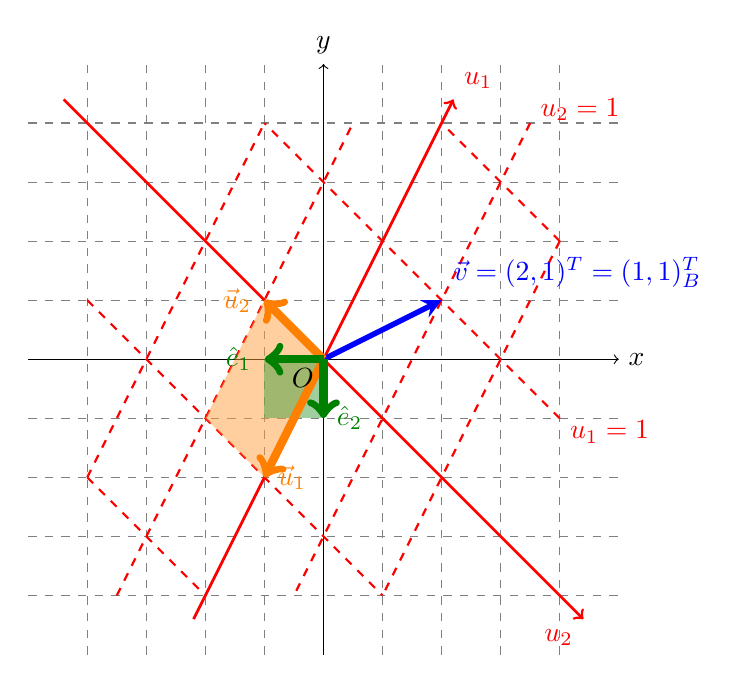
\begin{tikzpicture}[scale = 0.75]
\draw[->] (-5,0)--(5,0) node[right]{$x$};
\draw[->] (0,-5)--(0,5) node[above]{$y$};
\draw[gray,dashed] (-4,-5)--(-4,5);
\draw[gray,dashed] (-3,-5)--(-3,5);
\draw[gray,dashed] (-2,-5)--(-2,5);
\draw[gray,dashed] (-1,-5)--(-1,5);
\draw[gray,dashed] (4,-5)--(4,5);
\draw[gray,dashed] (3,-5)--(3,5);
\draw[gray,dashed] (2,-5)--(2,5);
\draw[gray,dashed] (1,-5)--(1,5);
\draw[gray,dashed] (-5,-4)--(5,-4);
\draw[gray,dashed] (-5,-3)--(5,-3);
\draw[gray,dashed] (-5,-2)--(5,-2);
\draw[gray,dashed] (-5,-1)--(5,-1);
\draw[gray,dashed] (-5,4)--(5,4);
\draw[gray,dashed] (-5,3)--(5,3);
\draw[gray,dashed] (-5,2)--(5,2);
\draw[gray,dashed] (-5,1)--(5,1);
\draw[red,->,line width=1] (-2.2,-4.4)--(2.2,4.4) node[above right]{$u_1$};
\draw[red,->,line width=1] (-4.4,4.4)--(4.4,-4.4) node[below left]{$u_2$};
\draw[red, thick, dashed] (4,-1)--(-1,4) node[right, pos=0, yshift=-5]{$u_1 = 1$};
\draw[red, thick, dashed] (3.5,4)--(-0.5,-4) node[right, pos=0, yshift=5]{$u_2 = 1$};
\draw[red, thick, dashed] (4,2)--(2,4);
\draw[red, thick, dashed] (4,2)--(1,-4);
\draw[red, thick, dashed] (-4,1)--(1,-4);
\draw[red, thick, dashed] (-4,-2)--(-2,-4);
\draw[red, thick, dashed] (-3.5,-4)--(0.5,4);
\draw[red, thick, dashed] (-4,-2)--(-1,4);
\draw[blue,-stealth,line width=2] (0,0)--(2,1) node[right, yshift=10]{$\vec{v} = (2,1)^T = (1,1)^T_B$};
\fill[orange!75, opacity=0.5] (0,0) -- (-1,1) -- (-2,-1) -- (-1,-2) -- cycle;
\fill[Green!75, opacity=0.5] (0,0) -- (-1,0) -- (-1,-1) -- (0,-1) -- cycle;
\draw[orange,->,line width=3] (0,0)--(-1,-2) node[right]{$\vec{u}_1$};
\draw[orange,->,line width=3] (0,0)--(-1,1) node[left]{$\vec{u}_2$};
\draw[Green,->,line width=3] (0,0)--(-1,0) node[left]{$\hat{e}_1$};
\draw[Green,->,line width=3] (0,0)--(0,-1) node[right]{$\hat{e}_2$};
\node[below left]{$O$}; 
\end{tikzpicture}
\end{center}
\end{solution}
In this example, we can see that in the two bases $\mathcal{S}$, $\mathcal{B}$, their axis vectors (reversed in the figure) can be transformed via $T: \mathbb{R}^2 \to \mathbb{R}^2$ with $T(\hat{e}_j) = \vec{u}_j$. The corresponding matrix representation is $\vec{u}_j = [\vec{u}_1|\vec{u}_2]\hat{e}_j = P_B^S\hat{e}_j$. Meanwhile the coordinate transformation follows $[\vec{v}]_B = (P_B^S)^{-1}[\vec{v}]_S = P_S^B[\vec{v}]_S$, where the transformation matrix is the inverse of the former. The former actually alters the vectors themselves and is sometimes known as an \index{Active Transformation}\keywordhl{active (coordinate) transformation}. In contrast, the latter only changes the coordinate frame but keep the vector unchanged and is hence called a \index{Passive Transformation}\keywordhl{passive (coordinate) transformation} (in fact, it is just the identity transformation with a change of basis). We can see that in the example above, after the active transformation the area of square formed by the new two basis vectors is enlarged by a factor of $\abs{\det(P_B^S)}=3$. Such a magnifying factor is a result of Properties \ref{proper:nvolume} and the similar holds for cases of any dimension. Oppositely, with the passive transformation we can say that the value of area of an identical square is shrinked to $\abs{\det(P_S^B)} = \abs{\det((P_B^S)^{-1})} = \abs{\det(P_B^S)}^{-1} = \frac{1}{3}$ of the original, expressed in the new units. Therefore, the appropriate factors in the two scenarios are the inverse of each other.

\subsubsection{Change of Coordinates for Linear Transformations/Matrices}

It is also possible to do a change of coordinates for linear transformations and hence the matrices that represent them. Consider a linear transformation $T: \mathcal{U} \to \mathcal{V}$ that has a matrix representation of $[\vec{v}]_H = [T]_B^H[\vec{u}]_B$ where $\mathcal{B}$ and $\mathcal{H}$ are bases for $\mathcal{U}$ and $\mathcal{V}$ respectively. If we want to change the basis for $\mathcal{U}$ from $\mathcal{B}$ to some other basis $\mathcal{B}'$ (and similarly $\mathcal{H}'$ for $\mathcal{V}$), then the new matrix representation of the linear transformation would be $[\vec{v}]_{H'} = [T]_{B'}^{H'}[\vec{u}]_{B'}$. Since they are the same transformation but only expressed in different coordinate systems, these two matrix equations have to be equivalent. Now, the vectors on both sides of the original equation themselves can undergo changes of coordinates according to the previous Theorem \ref{thm:bijectivechincoord} with $[\vec{u}]_B = [\text{id}]_{B'}^B [\vec{u}]_{B'} = P_{B'}^B [\vec{u}]_{B'}$ and $[\vec{v}]_{H} = [\text{id}]_{H'}^{H} [\vec{v}]_{H'} = Q_{H'}^H [\vec{v}]_{H'}$, where we denote the change of coordinates matrices from $\mathcal{B'}$ to $\mathcal{B}$ by $P_{B'}^{B}$ (and similarly  $\mathcal{H'}$ to $\mathcal{H}$ by $Q_{H'}^{H}$). Subsequently,
\begin{align*}
[\vec{v}]_H &= [T]_B^H[\vec{u}]_B \\
Q_{H'}^H [\vec{v}]_{H'} &= [T]_B^H P_{B'}^B [\vec{u}]_{B'} \\
[\vec{v}]_{H'} &= \left( (Q_{H'}^H)^{-1} [T]_B^H P_{B'}^B \right) [\vec{u}]_{B'}
\end{align*}
Comparing with the latter equation, we can identify $[T]_{B'}^{H'}$ with $(Q_{H'}^H)^{-1} [T]_B^H P_{B'}^B$, and this is the desired formula for change of coordinates over the matrix form of a linear transformation.
\begin{proper}
\label{proper:chcoordsmat}
The change of coordinates for the matrix representation of a linear transformation $T: \mathcal{U} \to \mathcal{V}$ from bases $\mathcal{B}$ and $\mathcal{H}$ to $\mathcal{B}'$ and $\mathcal{H}'$ for $\mathcal{U}$ and $\mathcal{V}$ respectively follows the relation
\begin{align*}
[T]_{B'}^{H'} = (Q_{H'}^H)^{-1} [T]_B^H P_{B'}^B
\end{align*}
where $P_{B'}^{B}$ and $Q_{H'}^{H}$ are matrices for change of coordinates on vectors from $\mathcal{B'}$ to $\mathcal{B}$ and $\mathcal{H'}$ to $\mathcal{H}$ individually.
\end{proper}
Another way to derive the above formula is to consider the linear transformation with respect to the basis $\mathcal{B'}$ to $\mathcal{H'}$ as three smaller steps: firstly, convert the input vector from the basis $\mathcal{B'}$ back to $\mathcal{B}$ ($P_{B'}^B$); subsequently, carry out the transformation in terms of $\mathcal{B}$ and $\mathcal{H}$ ($[T]_B^H$); finally, map the vector from the basis $\mathcal{H}$ to $\mathcal{H'}$ ($Q_H^{H'} = (Q_{H'}^H)^{-1}$). This flow is illustrated in the schematic of Figure \ref{fig:transcoordsmatrix}.
\begin{figure}
    \centering
    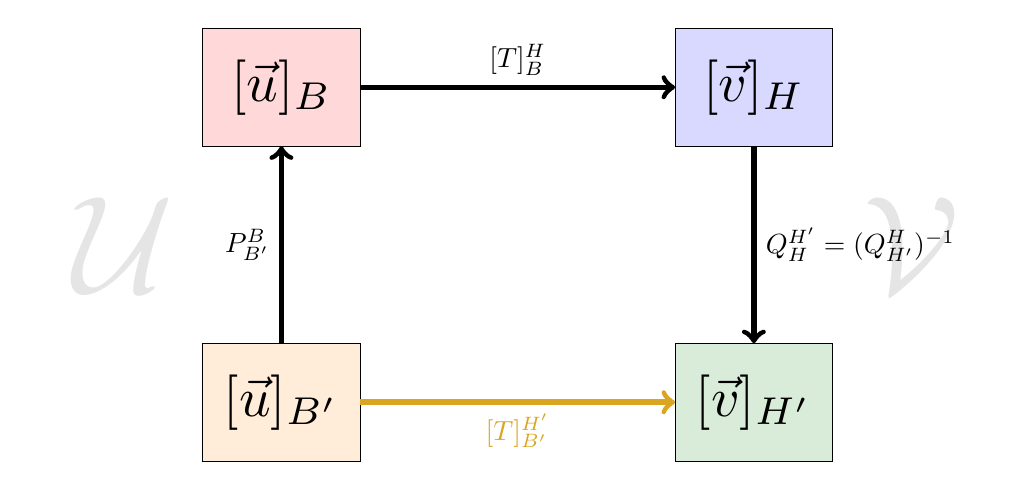
\begin{tikzpicture}
    \node[opacity=0.1,scale=5] at (-2,-2) {$\mathcal{U}$}; 
    \node[opacity=0.1,scale=5] at (8,-2) {$\mathcal{V}$};
    \draw [fill=red!15] (-1,-0.75) rectangle (1,0.75);
    \draw [fill=orange!15] (-1,-4.75) rectangle (1,-3.25);
    \draw [fill=blue!15] (5,-0.75) rectangle (7,0.75);
    \draw [fill=Green!15] (5,-4.75) rectangle (7,-3.25);
    \node[scale=2] at (0,0) {$[\vec{u}]_B$};
    \node[scale=2] at (6,0) {$[\vec{v}]_H$};
    \node[scale=2] at (0,-4) {$[\vec{u}]_{B'}$};
    \node[scale=2] at (6,-4) {$[\vec{v}]_{H'}$}; 
    \draw[->, line width=2] (0,-3.25) -- (0,-0.75) node[midway, left]{$P_{B'}^B$};
    \draw[->, line width=2] (6,-0.75) -- (6,-3.25) node[midway, right]{$Q_H^{H'} = (Q_{H'}^H)^{-1}$};
    \draw[->, line width=2] (1,0) -- (5,0) node[midway, above]{$[T]_B^H$};
    \draw[Goldenrod, ->, line width=2] (1,-4) -- (5,-4) node[midway, below]{$[T]_{B'}^{H'}$};
    \end{tikzpicture}
    \caption{A schematic showing how the change of coordinate bases works for linear transformation.}
    \label{fig:transcoordsmatrix}
\end{figure}

\begin{exmp}
Use Properties \ref{proper:chcoordsmat} to redo Example \ref{exmp:lineartransderivative} with respect to new bases $\mathcal{B}' = \{1, x-1, (x-1)^2\}$ and $\mathcal{H}' = \{1, x+1\}$.
\end{exmp}
\begin{solution}
First it is instructive to find $P_{B'}^B$ and $Q_{H'}^H$. We leave to the readers to verify that
\begin{align*}
P_{B'}^B &= 
\begin{bmatrix}
1 & -1 & 1 \\
0 & 1 & -2\\
0 & 0 & 1
\end{bmatrix}
& Q_{H'}^H &=
\begin{bmatrix}
1 & 1 \\
0 & 1 
\end{bmatrix}
\end{align*}
and hence by Properties \ref{proper:chcoordsmat},
\begin{align*}
[T]_{B'}^{H'} &= (Q_{H'}^H)^{-1} [T]_B^H P_{B'}^B \\
&= \begin{bmatrix}
1 & 1 \\
0 & 1 
\end{bmatrix}^{-1}
\begin{bmatrix}
0 & 1 & 0 \\
0 & 0 & 2
\end{bmatrix}
\begin{bmatrix}
1 & -1 & 1 \\
0 & 1 & -2\\
0 & 0 & 1
\end{bmatrix} \\
&= \begin{bmatrix}
1 & -1 \\
0 & 1 
\end{bmatrix}
\begin{bmatrix}
0 & 1 & 0 \\
0 & 0 & 2
\end{bmatrix}
\begin{bmatrix}
1 & -1 & 1 \\
0 & 1 & -2\\
0 & 0 & 1
\end{bmatrix} =
\begin{bmatrix}
0 & 1 & -4 \\
0 & 0 & 2
\end{bmatrix}
\end{align*}
We use a test case to check the answer. Let $p(x) = x^2 - 3x + 1 = (x-1)^2 - (x-1) - 1$. Then its coordinates in the $\mathcal{B}'$ basis is $(-1,-1,1)^T_{B'}$, and the transformation can be described by 
\begin{align*}
[T]_{B'}^{H'} (1,-1,-1)^T_{B'} &= 
\begin{bmatrix}
0 & 1 & -4 \\
0 & 0 & 2
\end{bmatrix}_{B'}^{H'}
\begin{bmatrix}
-1 \\
-1 \\
1
\end{bmatrix}_{B'}
=
\begin{bmatrix}
-5 \\
2
\end{bmatrix}_{H'}
\end{align*}
which corresponds to $-5(1) + 2(x+1) = 2x-3$, which is consistent with the usual calculation $T(p(x)) = p'(x) = (x^2-3x+1)' = 2x-3$ from elementary calculus.
\end{solution}

In most of the times, we are interested in the type of linear transformations that are an \index{Endomorphism}\keywordhl{endomorphism} (sometimes also referred to as a \index{Linear Operator}\keywordhl{linear operator}) in which the mapping is from a vector space $\mathcal{V}$ to itself, i.e. $T: \mathcal{V} \to \mathcal{V}$\footnote{An endomorphism that is at the same time an isomorphism is known as an \index{Automorphism}\keywordhl{automorphism}, e.g. the linear transformation in Example \ref{exmp:endomorphch}.}. Often we also use the same basis $\mathcal{B}$ for the input and output. Subsequently, to change the basis for both of them at the same time, let's say $\mathcal{B}'$, if the matrix for change of coordinates on vectors from $\mathcal{B}'$ to $\mathcal{B}$ is denoted as $P = P_{B'}^B$, then Properties \ref{proper:chcoordsmat} is reduced to $[T]_{B'}^{B'} = (P_{B'}^B)^{-1} [T]_B^B P_{B'}^B = P^{-1}AP$ where $A = [T]_B^B$ is the original matrix representation of the endomorphism. When it is clear from the context, we will simply write $[T]_B^B$ ($[T]_{B'}^{B'}$) as $[T]_B$ ($[T]_{B'}$).
\begin{proper}
\label{proper:endomorph}
For a linear endomorphism $T: \mathcal{V} \to \mathcal{V}$, the change of coordinates for its matrix representation from the old basis $\mathcal{B}$ to the new one $\mathcal{B}'$ is described by the formula
\begin{align*}
[T]_{B'} = (P_{B'}^B)^{-1} [T]_B P_{B'}^B    
\end{align*}
Or speaking loosely, the change of coordinates for a matrix in general takes the form of
\begin{align*}
A' = P^{-1}AP
\end{align*}
\end{proper}

\begin{exmp}
\label{exmp:endomorphch}
For a two-dimensional vector space $\mathcal{V}$ with a basis $\mathcal{B} = \{\vec{v}_1, \vec{v}_2\}$, if a linear endomorphism $T: \mathcal{V} \to \mathcal{V}$ is defined by $T(\vec{v}_1) = \vec{v}_1$, $T(\vec{v}_2) = \vec{v}_1 + \vec{v}_2$, finds its matrix representation with respect to $\mathcal{B}$. Subsequently, if a new basis $\mathcal{B}'$ is formed by $\{\vec{v}'_1, \vec{v}'_2\}$ where $\vec{v}'_1 = 2\vec{v}_1 - \vec{v}_2$ and $\vec{v}'_2 = -\vec{v}_1 + \vec{v}_2$, use Properties \ref{proper:endomorph} to compute the matrix representation of the endomorphism with respect to the new basis.
\end{exmp}
\begin{solution}
By Definition \ref{defn:matrixrepoflintrans}, the linear transformation has a matrix representation of
\begin{align*}
[T]_B = \begin{bmatrix}
[T(\vec{v}_1)]_B|[T(\vec{v}_2)]_B    
\end{bmatrix} &= 
\begin{bmatrix}
[\vec{v}_1]_B|[\vec{v}_1 + \vec{v}_2]_B    
\end{bmatrix} \\
&=
\begin{bmatrix}
1 & 1 \\
0 & 1
\end{bmatrix}
\end{align*}
with respect to the old basis $\mathcal{B}$. The appropriate $P_{B'}^B$ matrix that will be used for Properties \ref{proper:endomorph}, by Theorem \ref{thm:bijectivechincoord}, is
\begin{align*}
P_{B'}^B = 
\begin{bmatrix}
[\vec{v}'_1]_B|[\vec{v}'_2]_B
\end{bmatrix}
&= \begin{bmatrix}
[2\vec{v}_1 - \vec{v}_2]_B|[-\vec{v}_1 + \vec{v}_2]_B
\end{bmatrix} \\
&=
\begin{bmatrix}
2 & -1 \\
-1 & 1
\end{bmatrix}
\end{align*}
and thus the desired new matrix representation of the endomorphism with respect to $\mathcal{B}'$ is
\begin{align*}
[T]_{B'} &= (P_{B'}^B)^{-1} [T]_B P_{B'}^B \\
&= 
\begin{bmatrix}
2 & -1 \\
-1 & 1
\end{bmatrix}^{-1}
\begin{bmatrix}
1 & 1 \\
0 & 1
\end{bmatrix}
\begin{bmatrix}
2 & -1 \\
-1 & 1
\end{bmatrix} \\
&= 
\begin{bmatrix}
1 & 1 \\
1 & 2
\end{bmatrix}
\begin{bmatrix}
1 & 1 \\
0 & 1
\end{bmatrix}
\begin{bmatrix}
2 & -1 \\
-1 & 1
\end{bmatrix}
=
\begin{bmatrix}
0 & 1\\
-1 & 2
\end{bmatrix}
\end{align*}
\end{solution}

\subsection{Gram-Schmidt Orthogonalization, QR Decomposition}

Sometimes the coordinate basis consists of vectors that are linearly independent but not orthogonal to each other, unlike the standard basis. A common way to create an orthogonal basis from the set is to apply the so-called \index{Gram-Schmidt Orthogonalization}\keywordhl{Gram-Schmidt Orthogonalization}. Basically, it is an iterative method. At each step it constructs a vector that are orthogonal to all the previously processed vectors by removing the parallel components projected onto them (blue) while retaining the orthogonal part (red).
\begin{center}
\begin{tikzpicture}[scale=1.3]
\coordinate (0) at (0,0);
\coordinate (vecu) at (4,1);
\coordinate (vecv) at (1,2);
\draw[->](0)--(vecu) node[right]{$\vec{u}_1$, $\vec{v}_1$};
\draw[->](0)--(vecv) node[above]{$\vec{u}_2$};
\draw[red, dashed, thick, ->] (24/17, 6/17)--(1,2) node[midway, right]{$\vec{v_2}$};
\draw[red] (24/17+0.2, 6/17+0.05)--(24/17+0.15, 6/17+0.25)--(24/17-0.05, 6/17+0.2);
\pic[draw, "$\theta$", angle eccentricity=1.5] {angle = vecu--0--vecv};
\draw[blue, very thick] (0,0)--(24/17, 6/17) node[below, shift={(0mm, -2mm)}]{$\text{proj}_{v_1}\vec{u_2}$};
\end{tikzpicture}
\end{center}
\begin{defn}[Algorithm for Gram-Schmidt Orthogonalization]
\label{defn:GSorth}
Given a coordinate basis consisted of $\vec{u}_1, \vec{u}_2, \vec{u}_3, \ldots, \vec{u}_n \in \mathbb{R}^m$, Gram-Schmidt Orthogonalization transforms them into $\vec{v}_1, \vec{v}_2, \vec{v}_3, \ldots, \vec{v}_n \in \mathbb{R}^m$ ($m$ and $n$ are not necessarily equal) according to the following formulae:
\begin{align*}
\vec{v}_1 &= \vec{u}_1 \\
\vec{v}_2 &= \vec{u}_2 - \text{proj}_{v_1}\vec{u}_2 = \vec{u}_2 - \frac{\vec{v}_1 \cdot \vec{u}_2}{\norm{\vec{v}_1}^2} \vec{v}_1 \\
\vec{v}_3 &= \vec{u}_3 - \text{proj}_{v_1}\vec{u}_3 - \text{proj}_{v_2}\vec{u}_3 = \vec{u}_3 - \frac{\vec{v}_1 \cdot \vec{u}_3}{\norm{\vec{v}_1}^2} \vec{v}_1 - \frac{\vec{v}_2 \cdot \vec{u}_3}{\norm{\vec{v}_2}^2} \vec{v}_2 \\
\vdots \\
\vec{v}_n &= \vec{u}_n - \text{proj}_{v_1}\vec{u}_n - \text{proj}_{v_2}\vec{u}_n - \cdots - \text{proj}_{v_{n-1}}\vec{u}_n \\
&= \vec{u}_n - \frac{\vec{v}_1 \cdot \vec{u}_n}{\norm{\vec{v}_1}^2} \vec{v}_1 - \frac{\vec{v}_2 \cdot \vec{u}_n}{\norm{\vec{v}_2}^2} \vec{v}_2 - \cdots - \frac{\vec{v}_{n-1} \cdot \vec{u}_n}{\norm{\vec{v}_{n-1}}^2} \vec{v}_{n-1}
\end{align*}
In general, for $j \geq 2$, the $j$-th new vector is computed by
\begin{align*}
\vec{v}_j &= \vec{u}_j - \sum_{k=1}^{j-1}\text{proj}_{v_k}\vec{u}_j  = \vec{u}_j - \sum_{k=1}^{j-1}\frac{\vec{v}_k \cdot \vec{u}_j}{\norm{\vec{v}_k}^2} \vec{v}_k
\end{align*}
where the expression of projection, Properties \ref{proper:proj}, is used.
\end{defn}
A variant of Gram-Schmidt Orthogonalization is to normalize every vector at each step immediately, such that $\norm{\hat{v_j}} = 1$ for all $j$, and the resulted basis is said to be \index{Orthonormal}\keywordhl{orthonormal} (both orthogonal and of unit length). The formulae in Definition \ref{defn:GSorth} are then reduced to
\begin{defn}[Gram-Schmidt Orthogonalization with Normalization]
\label{defn:GSorth_norm}
\begin{align*}
\hat{v}_1 &= \frac{\vec{u}_1}{\norm{\vec{u}_1}} \\
\hat{v}_2 &= \frac{\vec{u}_2 - (\hat{v}_1 \cdot \vec{u}_2)\hat{v}_1}{\norm{\vec{u}_2 - (\hat{v}_1 \cdot \vec{u}_2)\hat{v}_1}} \\
\hat{v}_3 &= \frac{\vec{u}_3 - (\hat{v}_1 \cdot \vec{u}_3)\hat{v}_1 - (\hat{v}_2 \cdot \vec{u}_3)\hat{v}_2}{\norm{\vec{u}_3 - (\hat{v}_1 \cdot \vec{u}_3)\hat{v}_1 - (\hat{v}_2 \cdot \vec{u}_3)\hat{v}_2}} \\
\vdots \\
\hat{v}_n &= \frac{\vec{u}_n - (\hat{v}_1 \cdot \vec{u}_n)\hat{v}_1 - (\hat{v}_2 \cdot \vec{u}_n)\hat{v}_2 - \cdots - (\hat{v}_{n-1} \cdot \vec{u}_n)\hat{v}_{n-1}}{\norm{\vec{u}_n - (\hat{v}_1 \cdot \vec{u}_n)\hat{v}_1 - (\hat{v}_2 \cdot \vec{u}_n)\hat{v}_2 - \cdots - (\hat{v}_{n-1} \cdot \vec{u}_n)\hat{v}_{n-1}}} 
\end{align*}
For $j \geq 2$, the general formulae is
\begin{align*}
\hat{v}_j &= \frac{\vec{u}_j - \sum_{k=1}^{j-1}(\hat{v}_k \cdot \vec{u}_j)\hat{v}_k}{\norm{\vec{u}_j - \sum_{k=1}^{j-1}(\hat{v}_k \cdot \vec{u}_j)\hat{v}_k}}
\end{align*}
\end{defn}
\begin{exmp}
\label{exmp:GS_ex}
Perform Gram-Schmidt Orthogonalization with normalization on the coordinate basis for $\mathbb{R}^3$ that is consisted of $\vec{u_1} = (1,2,2)^T$, $\vec{u_2} = (1,-1,0)^T$, $\vec{u_3} = (3,-1,1)^T$, using the formula in Definition \ref{defn:GSorth_norm}.
\end{exmp}
\begin{solution}
The first vector is
\begin{align*}
\hat{v}_1 &= \frac{1}{\sqrt{1^2+2^2+2^2}}
\begin{bmatrix}
1 \\
2 \\
2
\end{bmatrix} 
= 
\frac{1}{3}
\begin{bmatrix}
1 \\
2 \\
2
\end{bmatrix} 
=
\begin{bmatrix}
\frac{1}{3} \\
\frac{2}{3} \\
\frac{2}{3}
\end{bmatrix}
\end{align*}
The second vector can be found via
\begin{align*}
\vec{u}_2 - (\hat{v}_1 \cdot \vec{u}_2)\hat{v}_1 &= 
\begin{bmatrix}
1 \\
-1 \\
0
\end{bmatrix} 
-
[(\frac{1}{3})(1) + (\frac{2}{3})(-1) + (\frac{2}{3})(0)]
\begin{bmatrix}
\frac{1}{3} \\
\frac{2}{3} \\
\frac{2}{3}
\end{bmatrix} \\
&= 
\begin{bmatrix}
1 \\
-1 \\
0
\end{bmatrix}
- (-\frac{1}{3})
\begin{bmatrix}
\frac{1}{3} \\
\frac{2}{3} \\
\frac{2}{3}
\end{bmatrix}
=
\begin{bmatrix}
\frac{10}{9} \\
-\frac{7}{9} \\
\frac{2}{9}
\end{bmatrix} \\
\hat{v_2} &= \frac{1}{\sqrt{(\frac{10}{9})^2+(-\frac{7}{9})^2+(\frac{2}{9})^2}}
\begin{bmatrix}
\frac{10}{9} \\
-\frac{7}{9} \\
\frac{2}{9}
\end{bmatrix}
=
\frac{3}{\sqrt{17}}
\begin{bmatrix}
\frac{10}{9} \\
-\frac{7}{9} \\
\frac{2}{9}
\end{bmatrix}
=
\begin{bmatrix}
\frac{10}{3\sqrt{17}} \\
-\frac{7}{3\sqrt{17}}\\
\frac{2}{3\sqrt{17}}
\end{bmatrix}
\end{align*}
By the same essence, we have the third vector as
\begin{align*}
&\quad \vec{u}_3 - (\hat{v}_1 \cdot \vec{u}_3)\hat{v}_1 - (\hat{v}_2 \cdot \vec{u}_3)\hat{v}_2\\
&=
\begin{bmatrix}
3 \\
-1 \\
1
\end{bmatrix}
-
[(\frac{1}{3})(3) + (\frac{2}{3})(-1) + (\frac{2}{3})(1)]
\begin{bmatrix}
\frac{1}{3} \\
\frac{2}{3} \\
\frac{2}{3}
\end{bmatrix} \\
&\quad -
[(\frac{10}{3\sqrt{17}})(3) + (-\frac{7}{3\sqrt{17}})(-1) + (\frac{2}{3\sqrt{17}})(1)]
\begin{bmatrix}
\frac{10}{3\sqrt{17}} \\
-\frac{7}{3\sqrt{17}} \\
\frac{2}{3\sqrt{17}}
\end{bmatrix} \\
&=
\begin{bmatrix}
3 \\
-1 \\
1
\end{bmatrix}
- 1
\begin{bmatrix}
\frac{1}{3} \\
\frac{2}{3} \\
\frac{2}{3}
\end{bmatrix}
-
\textcolor{red}{\frac{13}{\sqrt{17}}}
\begin{bmatrix}
\frac{10}{3\sqrt{17}} \\
-\frac{7}{3\sqrt{17}} \\
\frac{2}{3\sqrt{17}}
\end{bmatrix}
=
\begin{bmatrix}
\frac{2}{17} \\
\frac{2}{17} \\
-\frac{3}{17}
\end{bmatrix}
\\
\hat{v}_3 &=  \frac{1}{\sqrt{(\frac{2}{17})^2 + (\frac{2}{17})^2 + (-(\frac{3}{17}))^2}}
\begin{bmatrix}
\frac{2}{17} \\
\frac{2}{17} \\
-\frac{3}{17}
\end{bmatrix}
=
\textcolor{blue}{\sqrt{17}}
\begin{bmatrix}
\frac{2}{17} \\
\frac{2}{17} \\
-\frac{3}{17}
\end{bmatrix}
=
\begin{bmatrix}
\frac{2}{\sqrt{17}} \\
\frac{2}{\sqrt{17}} \\
-\frac{3}{\sqrt{17}}
\end{bmatrix}
\end{align*}
\end{solution}
Short Exercise: Verify that $\hat{v}_1, \hat{v}_2, \hat{v}_3$ are pairwise orthogonal.\footnote{We will only check $\hat{v}_1$ and $\hat{v}_3$ are orthogonal to each other and leave the remaining two pairs to the readers. $\hat{v}_1 \cdot \hat{v}_3 = (\frac{1}{3}, \frac{2}{3}, \frac{2}{3})^T \cdot (\frac{2}{\sqrt{17}}, \frac{2}{\sqrt{17}}, -\frac{3}{\sqrt{17}})^T = (\frac{1}{3})(\frac{2}{\sqrt{17}}) + (\frac{2}{3})(\frac{2}{\sqrt{17}}) + (\frac{2}{3})(-\frac{3}{\sqrt{17}}) = 0$.} \\
\\
An major application of the Gram-Schmidt process is the \index{QR Decomposition}\keywordhl{QR Decomposition}, which factors a matrix into two matrices, one as its orthogonal basis vectors arranged in columns and another one as a upper-triangular matrix (non-zero elements only found along or above the main diagonal) where the elements take the form of $\vec{u}_j \cdot \hat{v}_i$ as shown below. This is very useful in the processing of large matrices and least-square error fitting.
\begin{proper}
\label{proper:QRdecompose}
For a matrix $A = [\vec{u}_1|\vec{u}_2|\vec{u}_3|\cdots|\vec{u}_n]$, and the matrix $Q = [\hat{v}_1|\hat{v}_2|\hat{v}_3|\cdots|\hat{v}_n]$, where the $\hat{v}_j$ are orthonormal vectors that come from carrying out Gram-Schmidt orthogonalization on the basis vectors $\vec{u}_j$ according to the Definition \ref{defn:GSorth_norm}, we have $A = QR$, where
\begin{align*}
R &= 
\begin{bmatrix}
\hat{v}_1 \cdot \vec{u}_1 &  \hat{v}_1 \cdot \vec{u}_2 & \hat{v}_1 \cdot \vec{u}_3 & \cdots & \hat{v}_1 \cdot \vec{u}_n \\
0 & \hat{v}_2 \cdot \vec{u}_2 &  \hat{v}_2 \cdot \vec{u}_3 &  & \hat{v}_2 \cdot \vec{u}_n \\
0 & 0 & \hat{v}_3 \cdot \vec{u}_3 &  & \hat{v}_3 \cdot \vec{u}_n \\
\vdots & & & \ddots & \vdots\\
0 & 0 & 0 & \cdots & \hat{v}_n\cdot \vec{u}_n \\
\end{bmatrix} \\
\text{i.e. } R_{ij} &= 
\begin{cases}
\hat{v}_i \cdot \vec{u}_j & i \leq j \\
0 & i > j
\end{cases}
& \text{for $1 \leq i, j \leq n$}
\end{align*}
is an upper triangular $n \times n$ invertible matrix.
\end{proper}
\begin{proof}
We will show that every column of $A$ and $QR$ coincides. The $j$-th column of $A$ is simply the $j$-th vector in the starting basis, $\vec{u}_j$. Meanwhile, the $j$-th column of $QR$ is $Q$ times the $j$-th column of $R$, which is
\begin{align*}
QR^{(j)} &=
\begin{bmatrix}
\hat{v}_1|\hat{v}_2|\cdots|\hat{v}_j|\cdots|\hat{v}_n   
\end{bmatrix}
\begin{bmatrix}
\hat{v}_1 \cdot \vec{u}_j \\   
\hat{v}_2 \cdot \vec{u}_j \\   
\vdots \\
\hat{v}_j \cdot \vec{u}_j \\
\vdots \\
0
\end{bmatrix} \\
&= (\hat{v}_1 \cdot \vec{u}_j) \hat{v}_1 + (\hat{v}_2 \cdot \vec{u}_j) \hat{v}_2 + \cdots + (\hat{v}_j \cdot \vec{u}_j) \hat{v}_j + 0 \\
&= \sum_{k=1}^{j}(\hat{v_k} \cdot \vec{u_j})\hat{v_k} = \sum_{k=1}^{j-1}(\hat{v_k} \cdot \vec{u_j})\hat{v_k} + (\hat{v_j} \cdot \vec{u_j})\hat{v_j}
\end{align*}
By Definition \ref{defn:GSorth_norm}, we have
\begin{align*}
\hat{v}_j &= \frac{\vec{u}_j - \sum_{k=1}^{j-1}(\hat{v}_k \cdot \vec{u}_j)\hat{v}_k}{\norm{\vec{u}_j - \sum_{k=1}^{j-1}(\hat{v}_k \cdot \vec{u}_j)\hat{v}_k}}
\end{align*}
\footnote{\label{foot:GSnonzero} Some may ask if $\norm{\vec{u}_j - \sum_{k=1}^{j-1}(\hat{v}_k \cdot \vec{u}_j)\hat{v}_k}$ can be $0$ (or $\vec{u}_j - \sum_{k=1}^{j-1}(\hat{v}_k \cdot \vec{u}_j)\hat{v}_k$ be the zero vector) and $\hat{v}_j$ is not well-defined. However, this will contradict the linear independence of the basis vectors $\vec{u}_k$. We can use induction to show this: (WIP)} which after rearrangement, becomes
\begin{align*}
\vec{u}_j = \sum_{k=1}^{j-1}(\hat{v}_k \cdot \vec{u}_j)\hat{v}_k + {\norm{\vec{u}_j - \sum_{k=1}^{j-1}(\hat{v}_k \cdot \vec{u}_j)\hat{v}_k}}\hat{v}_j
\end{align*}
Therefore, in order to show that $\vec{u}_j = QR^{(j)}$, by comparing the two expressions, we need to check if
\begin{align*}
\hat{v}_j \cdot \vec{u}_j &= {\norm{\vec{u}_j - \sum_{k=1}^{j-1}(\hat{v}_k \cdot \vec{u}_j)\hat{v}_k}} 
\end{align*}
Consider
\begin{align*}
(\vec{u}_j - \sum_{k=1}^{j-1}(\hat{v}_k \cdot \vec{u}_j)\hat{v}_k) \cdot \hat{v}_j &= \hat{v}_j \cdot \vec{u}_j - \sum_{k=1}^{j-1}(\hat{v}_k \cdot \vec{u_j}) (\hat{v}_k \cdot \hat{v}_j)\\
&= \hat{v}_j \cdot \vec{u}_j 
\end{align*}
as $\vec{v}_k \cdot \hat{v}_j = 0$ for $k \neq j$ due to the orthogonality enforced by the Gram-Schmidt process. On the other hand, by Definition \ref{defn:GSorth_norm} again, 
\begin{align*}
\vec{u}_j - \sum_{k=1}^{j-1}(\hat{v}_k \cdot \vec{u}_j)\hat{v}_k = \norm{\vec{u}_j - \sum_{k=1}^{j-1}(\hat{v}_k \cdot \vec{u}_j)\hat{v}_k} \hat{v}_j
\end{align*}
Therefore,
\begin{align*}
(\vec{u}_j - \sum_{k=1}^{j-1}(\hat{v}_k \cdot \vec{u}_j)\hat{v}_k) \cdot \hat{v}_j &= \left(\norm{\vec{u}_j - \sum_{k=1}^{j-1}(\hat{v}_k \cdot \vec{u}_j\hat{v}_k} \hat{v}_j)\right) \cdot \hat{v}_j \\
&= \norm{\vec{u}_j - \sum_{k=1}^{j-1}(\hat{v}_k \cdot \vec{u}_j)\hat{v}_k} (\hat{v}_j \cdot \hat{v}_j) \\
&= \norm{\vec{u}_j - \sum_{k=1}^{j-1}(\hat{v}_k \cdot \vec{u}_j)\hat{v}_k}
\end{align*}
as $\hat{v}_j \cdot \hat{v}_j = \norm{\hat{v}_j}^2 = 1^2 = 1$. The required equality is then established and the result follows. The invertibility of $R$ can be shown by noting that all diagonal elements $\hat{v}_j \cdot \hat{u}_j = {\norm{\vec{u}_j - \sum_{k=1}^{j-1}(\hat{v}_k \cdot \vec{u}_j)\hat{v}_k}} $ of the upper triangular $R$ matrix are non-zero (see Footnote \ref{foot:GSnonzero}). 
\end{proof}

\begin{exmp}
\label{exmp:QRdecom}
Construct a QR decomposition for the case in Example \ref{exmp:GS_ex}.
\end{exmp}
\begin{solution}
The matrix $Q$ is simply
\begin{align*}
Q &= 
\begin{bmatrix}
\frac{1}{3} & \frac{10}{3\sqrt{17}} & \frac{2}{\sqrt{17}} \\
\frac{2}{3} & -\frac{7}{3\sqrt{17}} & \frac{2}{\sqrt{17}} \\
\frac{2}{3} & \frac{2}{3\sqrt{17}} & -\frac{3}{\sqrt{17}}
\end{bmatrix}
\end{align*}
And by Properties \ref{proper:QRdecompose}, the entries in $R$ are
\begin{align*}
R &= 
\begin{bmatrix}
\hat{v}_1 \cdot \vec{u}_1 &  \hat{v}_1 \cdot \vec{u}_2 & \hat{v}_1 \cdot \vec{u}_3 \\
0 & \hat{v}_2 \cdot \vec{u}_2 &  \hat{v}_2 \cdot \vec{u}_3 \\
0 & 0 & \hat{v}_3 \cdot \vec{u}_3 
\end{bmatrix}  \\
&= 
\begin{bmatrix}
3 & -\frac{1}{3} & 1 \\
0 & \frac{\sqrt{17}}{3} & \textcolor{red}{\frac{13}{\sqrt{17}}}  \\
0 & 0 & \textcolor{blue}{\frac{1}{\sqrt{17}}} \\
\end{bmatrix} 
\end{align*}
whose values can be readily inferred from the steps during the orthogonalization process itself in Example \ref{exmp:GS_ex} (highlighted in red/blue). The readers are encouraged to compute the matrix product $QR$ to see if the original matrix $A$ is recovered.\\
\\
We conclude this section with a small remark related to the concept of orthogonal complement discussed in Section \ref{section:null}.
\begin{proper}
For an orthogonal(-normal) basis $\mathcal{B} = \{\vec{v}_1, \vec{v}_2, \vec{v}_3, \cdots, \vec{v}_n\}$ for a finite-dimensional vector space $\mathcal{V}$, the subspaces $\mathcal{V}_G$ and $\mathcal{V}_H$ formed by $\mathcal{G} = \{\vec{v}_I\}$ and $\mathcal{H} = \{\vec{v}_J\}$ respectively, where $I$ and $J$ are mutually exclusive indices that together exhaust all integers from $1$ to $n$, are the orthogonal complement to each other, such that $\mathcal{V}_G^\perp = \mathcal{V}_H$ and $\mathcal{V}_G \oplus \mathcal{V}_H = \mathcal{V}$.
\end{proper}
\end{solution}

\section{Python Programming}
We can define a function to a change in coordinates for vectors or matrices. Let's first write a helper function to produce the change of coordinates matrix $P$ proposed in Theorem \ref{thm:bijectivechincoord}, which equals to $B'^{-1}B$ as discussed in the end of Example \ref{exmp:changecoord}:
\begin{lstlisting}
import numpy as np
from scipy import linalg

def P_matrix(B, B_prime):
    """ Computes the P matrix of change in coordinates. """
    P = linalg.inv(B_prime) @ B
    return(P)
\end{lstlisting}
Then we use Example \ref{exmp:2Dtransform} as an illustration for coordinate change for vectors, where regarding $\mathcal{B}$ we have
\begin{align*}
B = 
\begin{bmatrix}
1 & 1 \\ 
2 & -1
\end{bmatrix}
\end{align*}
and $B' = I$ as $\mathcal{B}' = \mathcal{S}$ implicitly in this case. We define another function for transforming the coordinates of any given vector as
\begin{lstlisting}
def coord_trans_vector(vec, P):
    """ Transforms the coordinates of a vector. """
    trans_vec = linalg.inv(P) @ vec
    return(trans_vec)    
\end{lstlisting}
Then Example \ref{exmp:2Dtransform} can be proceeded as follows.
\begin{lstlisting}
B = np.array([[1.,  1.], 
              [2., -1.]])

P = P_matrix(B, np.identity(2))
old_v = np.array([2., 1.])
new_v = coord_trans_vector(old_v, P)
print(new_v)    
\end{lstlisting}
which returns \verb|[1. 1.]| correctly. Similarly, according to Properties \ref{proper:endomorph}, we can make a function to carry out the change of coordinates for matrices through
\begin{lstlisting}
def coord_trans_matrix(A, P):
    """ Transforms the coordinates of a matrix. """
    trans_matrix = linalg.inv(P) @ A @ P
    return(trans_matrix)    
\end{lstlisting}
Let's use this to redo Example \ref{exmp:endomorphch}, where
\begin{align*}
A &= 
\begin{bmatrix}
1 & 1 \\
0 & 1
\end{bmatrix} &
& P=
\begin{bmatrix}
2 & -1 \\
-1 & 1
\end{bmatrix}
\end{align*}
Subsequently,
\begin{lstlisting}
B = np.array([[2., -1.], 
             [-1.,  1.]])
old_A = np.array([[1.,  1.], 
              [0.,  1.]])

P = P_matrix(B, np.identity(2))
new_A = coord_trans_matrix(old_A, P)
print(new_A)    
\end{lstlisting}
gives
\begin{lstlisting}
[[ 0.  1.]
 [-1.  2.]]    
\end{lstlisting}
as expected. Meanwhile, to apply Gram-Schmidt Orthogonalization for a basis, in addition to deriving the corresponding QR decomposition, we can use the function \verb|qr| in \verb|scipy.linalg|. Let's we use Examples \ref{exmp:GS_ex} and \ref{exmp:QRdecom} as a demonstration:
\begin{lstlisting}
A = np.array([[1.,  1.,  3.],
              [2., -1., -1.],
              [2.,  0.,  1.],])
Q, R = linalg.qr(A)
print("Q = ", Q)
print("R = ", R)
\end{lstlisting}
which yields
\begin{lstlisting}
Q =  [[-0.33333333  0.80845208 -0.48507125]
      [-0.66666667 -0.56591646 -0.48507125]
      [-0.66666667  0.16169042  0.72760688]]
R =  [[-3.          0.33333333 -1.        ]
      [ 0.          1.37436854  3.15296313]
      [ 0.          0.         -0.24253563]]
\end{lstlisting}
The columns in \verb|Q| form the desired orthonormal basis. Notice that the signs of the first/third column vectors in \verb|Q| are flipped when compared to that in Example \ref{exmp:QRdecom}, which leads to corresponding sign switches in \verb|R| as well.

\section{Exercises}

\begin{Exercise}
Let $\mathcal{V} = \mathcal{W} = \mathbb{R}^3$, and take $\mathcal{B} = \{(1,1,1)^T, (1,1,0)^T, (1,0,0)^T\}$ and $\mathcal{H} = \{(1,2,3)^T, (1,-1,0)^T, (2,-1,-1)^T\}$ as bases for $\mathcal{V}$ and $\mathcal{W}$. If a linear transformation $T: \mathbb{R}^3 \to \mathbb{R}^3$ is defined by $T(x,y,z)^T = (x+y+z,2x+y,x-y-3z)^T$, find its matrix representation and decide if it is one-to-one, onto and hence bijective.
\end{Exercise}

\begin{Exercise}
Let $\mathcal{V}$ be the real vector space generated by the basis $\mathcal{B} = \{\cos x, \sin x, x\cos x, x\sin x\}$ and $T: \mathcal{V} \to \mathcal{V}, T[f(x)] = f'(x)$ be the differentiation operator over $\mathcal{V}$. Find the matrix representation of $T$ with respect to $\mathcal{B}$, and determine if $T$ is injective, surjective and hence bijective. 
\end{Exercise}

\begin{Exercise}
Let $\mathcal{V} = \mathcal{P}^2$, $\mathcal{W} = \mathcal{P}^3$ be the polynomial spaces of degree $2$ and $3$ respectively. Define $T: \mathcal{V} \to \mathcal{W}$ by
\begin{align*}
T[p(x)] = \int_1^x p(x) dx
\end{align*}
find its matrix representation with respect to the standard bases and decide if the transformation is isomorphic.
\end{Exercise}

\begin{Exercise}
Show that every identity transformation $T: \mathcal{V} \to \mathcal{V}, T(\vec{v}) = \text{id}(\vec{v}) = \vec{v}$ for a finite-dimensional vector space $\mathcal{V}$ with respect to a fixed basis $\mathcal{B}$ throughout always has a matrix representation of an identity matrix such that $[T]_B = I$. 
\end{Exercise}

\begin{Exercise}
Apply Gram-Schmidt Orthogonalization on the following set of vectors, and then write down their QR Decomposition.
\begin{enumerate}[label=(\alph*)]
\item $\vec{u}_1 = (1,2)^T, \vec{u}_2 = (3,8)^T$,
\item $\vec{u}_1 = (1,2,1)^T, \vec{u}_2 = (1,4,4)^T, \vec{u}_3 = (2,2,5)^T$, and
\item $\vec{u}_1 = (1,-2,2,1)^T, \vec{u}_2 = (1,1,0,2)^T, \vec{u}_3 = (2,3,-1,0)^T$.
\end{enumerate}  
\end{Exercise}